%%% The main file. It contains definitions of basic parameters and includes all other parts.

%% Settings for single-side (simplex) printing
% Margins: left 40mm, right 25mm, top and bottom 25mm
% (but beware, LaTeX adds 1in implicitly)
\documentclass[12pt,a4paper]{report}
\setlength\textwidth{145mm}
\setlength\textheight{247mm}
\setlength\oddsidemargin{15mm}
\setlength\evensidemargin{15mm}
\setlength\topmargin{0mm}
\setlength\headsep{0mm}
\setlength\headheight{0mm}
% Recommended layout mentions line spacing 1.5, but this is not relevant to TeX.
% \openright makes the following text appear on a right-hand page
\let\openright=\clearpage

%% Settings for two-sided (duplex) printing
% \documentclass[12pt,a4paper,twoside,openright]{report}
% \setlength\textwidth{145mm}
% \setlength\textheight{247mm}
% \setlength\oddsidemargin{14.2mm}
% \setlength\evensidemargin{0mm}
% \setlength\topmargin{0mm}
% \setlength\headsep{0mm}
% \setlength\headheight{0mm}
% \let\openright=\cleardoublepage

\usepackage[utf8]{inputenc}

\usepackage{algorithmicx}
\usepackage{algpseudocode}
\usepackage{amsmath}           % \text{} in mathmode
\usepackage{amssymb}
\usepackage{authoraftertitle}
\usepackage{graphicx}          % Embedded graphics
\usepackage[numbers]{natbib}   % Bibliography
\usepackage{rotating}          % sidewaystable env in Results chapter
\usepackage{siunitx}           % Decimal-aligned tables in Results chapter
\usepackage{subcaption}        % Sub-figures
\usepackage{textcomp}          % \textdegree
\usepackage{gensymb}           % \degree in math
\usepackage{ucs}               % Refer to Unicode symbols by codepoint
\usepackage{url}

\usepackage{amsthm}            % Theorems, definitions, proofs
\newtheorem{theorem}{Theorem}
\newtheorem{lemma}{Lemma}
\newtheorem*{define}{Definition}	% Definice nečíslujeme, proto "*"

\usepackage{listings}          % Code listings
\lstset{
	basicstyle=\footnotesize\ttfamily,
	frame=single
}

\usepackage{tikz}              % Drawings embedded in LaTeX
\usetikzlibrary{calc, shapes, fit, positioning, matrix}

%% Custom commands
\newcommand{\E}{\mathbb{E}}
\newcommand{\Var}{\mathrm{Var}}
% Hyperfloors are defined by package 'nath', but it's not compatible with TikZ
\def\hyperspc{\kern -0.22em}
\newcommand{\lhfloor}{\lfloor \hyperspc \lfloor}
\newcommand{\rhfloor}{\rfloor \hyperspc \rfloor}
\newcommand{\Cpp}{C\texttt{++}}

%%% Basic information on the thesis

% Thesis title in English (exactly as in the formal assignment)
\title{Practical data structures}
% Author of the thesis
\author{Michael Pokorný}

% Year when the thesis is submitted
\def\YearSubmitted{2015}

% Name of the department or institute, where the work was officially assigned
% (according to the Organizational Structure of MFF UK in English,
% or a full name of a department outside MFF)
\def\Department{Department of Applied Mathematics}

% Is it a department (katedra), or an institute (ústav)?
\def\DeptType{Department}

% Thesis supervisor: name, surname and titles
\def\Supervisor{Mgr. Martin Mareš, Ph.D.}

% Supervisor's department (again according to Organizational structure of MFF)
\def\SupervisorsDepartment{Department of Applied Mathematics}

% Study programme and specialization
\def\StudyProgramme{Computer science}
\def\StudyBranch{General computer science}

% An optional dedication: you can thank whomever you wish (your supervisor,
% consultant, a person who lent the software, etc.)
\def\Dedication{%
	I~wish to express my thanks to my advisor, Martin ``MJ'' Mareš,
	and everyone who ever organized or will organize the KSP seminar,
	for mentoring not only myself, but also countless other aspiring
	computer scientists over many years. I~also thank my awesome parents
	and my awesome friends for being awesome.
}

% Abstract (recommended length around 80-200 words; this is not a copy of your thesis assignment!)
\def\Abstract{%
	In this thesis, we implement several common and uncommon
	data structures for ordered and unordered dictionaries and we benchmark
	their performance in main memory.

	To illustrate the importance of cache-aware design in modern computers,
	we benchmark hand-optimized \mbox{B-trees} against more traditional data
	structures (red-black trees and hashing).
	Cache-oblivious algorithms can take advantage of the memory hierarchy
	without explicit hand-tuning. We also implemented a cache-oblivious
	equivalent of \mbox{B-trees} and compared its performance to hand-tuned
	\mbox{B-trees}.

	Self-adjusting data structures, like splay trees, are difficult to
	reconcile with block operations in a memory hierarchy: for example,
	splay trees perform $\O(\log N)$ amortized memory reads from
	unpredictable locations on every \textsc{Find}, where \mbox{B-trees}
	only need $\O(\log_B N)$ cache misses.
	Splay trees are probably the most common self-adjusting dictionary.
	We compare their performance with non-self-adjusting structures and
	with more exotic self-adjusting structures designed for block memory
	access ($k$-forests and $k$-splay trees).
}

% 3 to 5 keywords (recommended), each enclosed in curly braces
\def\Keywords{
	{cache-oblivious algorithms}, {data structures}, {dictionaries},
	{search trees}
}

%% The hyperref package for clickable links in PDF and also for storing
%% metadata to PDF (including the table of contents).
\usepackage[pdftex,unicode]{hyperref}   % Must follow all other packages
\hypersetup{breaklinks=true}
\hypersetup{pdftitle={\MyTitle}}
\hypersetup{pdfauthor={\MyAuthor}}
\hypersetup{pdfkeywords=\Keywords}

% Slimejzi. FIXME: Remove before printing (should be fairly obvious).
%\overfullrule=2cm

\def\O{\mathcal{O}}  % \O is already taken by crossed O
\def\Z{\mathbb{Z}}

%%% Minor tweaks of style

% These macros employ a little dirty trick to convince LaTeX to typeset
% chapter headings sanely, without lots of empty space above them.
% Feel free to ignore.
\makeatletter
\def\@makechapterhead#1{
  {\parindent \z@ \raggedright \normalfont
   \Huge\bfseries \thechapter. #1
   \par\nobreak
   \vskip 20\p@
}}
\def\@makeschapterhead#1{
  {\parindent \z@ \raggedright \normalfont
   \Huge\bfseries #1
   \par\nobreak
   \vskip 20\p@
}}
\makeatother

% This macro defines a chapter, which is not numbered, but is included
% in the table of contents.
\def\chapwithtoc#1{
\chapter*{#1}
\addcontentsline{toc}{chapter}{#1}
}

\begin{document}

%%% Title page of the thesis and other mandatory pages
% Somewhat relaxed hyphenation
\lefthyphenmin=2
\righthyphenmin=2

%%% Title page of the thesis

\pagestyle{empty}
\hypersetup{pageanchor=false}
\begin{center}

\large

Charles University in Prague

\medskip

Faculty of Mathematics and Physics

\vfill

{\bf\Large BACHELOR THESIS}

\vfill

\centerline{\mbox{\includegraphics[width=60mm]{img/logo.eps}}}

\vfill
\vspace{5mm}

{\LARGE\MyAuthor}

\vspace{15mm}

{\LARGE\bfseries\MyTitle}

\vfill

\Department

\vfill

\begin{tabular}{rl}

Supervisor of the bachelor thesis: & \Supervisor \\
\noalign{\vspace{2mm}}
Study programme: & \StudyProgramme \\
\noalign{\vspace{2mm}}
Study branch: & \StudyBranch \\
\end{tabular}

\vfill

Prague \YearSubmitted

\end{center}

\newpage

%%% Here should be a bound sheet included -- a signed copy of the "bachelor
%%% thesis assignment". This assignment is NOT a part of the electronic
%%% version of the thesis. DO NOT SCAN.

%%% A page with a solemn declaration to the bachelor thesis

\openright
\hypersetup{pageanchor=true}
\pagestyle{plain}
\pagenumbering{roman}
\vglue 0pt plus 1fill

\noindent
I declare that I carried out this bachelor thesis independently, and only with the cited
sources, literature and other professional sources.

\medskip\noindent
I understand that my work relates to the rights and obligations under the Act No.~121/2000 Sb.,
the Copyright Act, as amended, in particular the fact that the Charles
University in Prague has the right to conclude a license agreement on~the~use of this
work as a school work pursuant to Section 60 subsection 1 of~the~Copyright Act.

\vspace{20mm}

\hbox{\hbox to 0.7\hsize{%
In \makebox[3cm]{\dotfill} date \makebox[3cm]{\dotfill}
\hss}\hbox to 0.3\hsize{%
signature of the author
\hss}}

\vspace{20mm}
\newpage

%%% Mandatory information page of the thesis

\openright

\vbox to 0.5\vsize{
\setlength\parindent{0mm}
\setlength\parskip{5mm}

Title:
\MyTitle

Author:
\MyAuthor

\DeptType:
\Department

Supervisor:
\Supervisor, \SupervisorsDepartment

Abstract:
\Abstract

Keywords:
\Keywords

\vss}

\newpage

%%% Dedication

\openright

\noindent
\Dedication

\newpage

\openright
\pagestyle{plain}
\pagenumbering{arabic}
\setcounter{page}{1}


%%% A page with automatically generated content of the bachelor thesis. For
%%% a mathematical thesis, it is permissible to have a list of tables and abbreviations,
%%% if any, at the beginning of the thesis instead of at its end.

\tableofcontents

%%% Each chapter is kept in a separate file
\chapter*{Introduction}
\addcontentsline{toc}{chapter}{Introduction}

It is a well-known fact that there is a widening gap between
the performance of CPUs and memory. To optimize memory accesses,
modern computers include several small and fast caches between the CPU and
main memory. However, if programs access data mostly randomly, I/O can become
the performance bottleneck, even for programs running only in main memory.

Standard models of computation only measure the performance of algorithms
in the number of CPU instructions executed and the number of memory cells used.
These models aren't well suited for environments where different memory cells
may have vastly different access speeds, for example depending on which caches
currently hold the particular memory cell. The \emph{external memory model}
is a simple extension of the RAM model that is better suited for analyzing
algorithms in memory hierarchies. This model adds a \emph{block transfer}
measure, which is the number of \emph{blocks} transferred between a fast cache
and a slow \emph{external memory}.
While the original motivation was developing fast algorithms for data stored on
hard drives, the model can also be used to reason about boundaries between
internal memory and caches.

\emph{Cache-oblivious algorithms} are a class of external memory algorithms
that perform equally well given any cache size and block size. Thanks to this
property, they need little tuning for efficient implementation.
Modern CPU architectures perform various optimizations that can change
the effective size of a block, so tuning an algorithm by setting a good block
size might be difficult.
The external memory model and cache-oblivious algorithms are introduced in more
detail in chapter~\ref{chapter:models}.

This thesis explores the performance implications of memory hierarchies
on data structures implementing dictionaries or sorted dictionaries.
Especially unsorted dictionaries are very useful in practice, as illustrated
by modern programming languages, which frequently reserve a built-in
data type for unsorted dictionaries (e.g.,\ \texttt{std::unordered\_map} in
\Cpp, \texttt{dict} in Python, or hashes in Perl).

Dictionaries maintain a set of $N$ key-value pairs with distinct keys.
Denote the set of stored keys by $K$.
The \textsc{Find} operation find the value associated with a~given key, or
it reports that no such value exists. \textsc{Insert} inserts a new
key-value pair and \textsc{Delete} removes a key-value pair given its key.
Sorted dictionaries additionally maintain an ordering on the keys and they
allow \textsc{FindNext} and \textsc{FindPrevious} operations.
Given a key $k$, which may or may not be present in the dictionary,
\textsc{FindNext} and \textsc{FindPrevious} find the closest larger or smaller
key present in the dictionary.

We implemented and benchmarked several common and uncommon data structures
for sorted and unsorted dictionaries. Our choice of data structures was
intended to sample simple dictionaries for RAM, cache-friendly dictionaries
for external memory and self-adjusting structures.
A high-level description of our implementation and benchmarks is presented
in chapter \ref{chapter:implementation}. The results are discussed in
chapter \ref{chapter:results}.

The most common data structure implementing an unsorted dictionary is a~hash
table. We describe some variants of hash tables in chapter \ref{chapter:hashing}.
Most hash tables have expected $\O(1)$ time for all operations, which
makes them quite practical. On the other hand, there is no simple way to
implement sorted dictionaries efficiently via hash tables.

Ordered dictionaries are usually maintained in search trees.
AVL trees, red-black trees and B-trees are examples of \emph{balanced search
trees}: a design invariant maintains their height low. The speeds
of \textsc{Find}, \textsc{Insert} and \textsc{Delete} mostly depend
on the number of nodes touched by the operations, which is $\Theta(h)$, where
$h$ is the height of the tree. AVL trees and red-black trees are binary, so
$h=\Theta(\log N)$. B-trees store $\Theta(b)$ keys per node, where $b\geq 2$,
and they maintain all leaves at the same depth, so operations on B-trees
touch $\Theta(\log_b N)$ nodes.

Splay trees are binary search trees with a self-adjusting rule, but splay
trees are not balanced, as this rule does not guarantee a small height in all
cases. The structure of a splay tree depends not only on the sequence of
\textsc{Insert}s and \textsc{Delete}s, but also on executed \textsc{Find}s.
The self-adjusting rule (\emph{splaying}) puts recently accessed nodes
near the root, so \textsc{Find}s on frequently or recently accessed keys
are faster than in balanced trees. On the other hand, splaying can put
the splay tree in a~degenerate state, in which accessing an unlucky node
touches $\Theta(N)$ nodes. Fortunately, the amortized number of node
reads per \textsc{Find} turns out to be $\O(\log N)$.

Splay trees are good at storing nonuniformly accessed dictionaries, but
the expected number of nodes read to \textsc{Find} a key is generally a factor
of $\Theta(\log b)$ higher than in B-trees. We briefly introduce two
self-adjusting data structures designed for both exploiting non-uniform
access patterns and to perform less I/O: \emph{$k$-splay trees} in chapter
\ref{chapter:ksplay} and \emph{$k$-forests} in chapter \ref{chapter:kforest}.

In chapter \ref{chapter:cob}, we describe \emph{cache-oblivious B-trees}.
The number of memory operations for cache-oblivious B-tree operations
is within a constant factor of the bounds given by a B-tree optimally tuned
for the memory hierarchy. In practice, we found the performance of
cache-oblivious B-trees quite competitive, especially on large datasets
with uniform access patterns.

The chapters on hashing and cache-oblivious B-trees are based on the Advanced
Data Structures course as taught by Erik Demaine on MIT in spring 2012.
Lecture videos and other materials are available through MIT OpenCourseWare.\footnote{%
\url{http://ocw.mit.edu/courses/electrical-engineering-and-computer-science/6-851-advanced-data-structures-spring-2012/index.htm}}

\section*{Notation and conventions}
In this thesis, logarithms are in base 2 unless stated otherwise.
Chapter \ref{chapter:cob} uses the \emph{hyperfloor} operation
$\lhfloor x\rhfloor$, which is defined as $2^{\lfloor\log x\rfloor}$.

We denote bitwise XOR as $\oplus$, and similarly $\bigoplus_{i=1}^N
a_i=a_1\oplus\ldots\oplus a_N$.

This thesis contains several references to memory sizes. The base units of
memory size are traditionally powers of two to simplify some operations on
addresses.
When discussing memory, we shall follow this convention, so
$1\ \mathrm{kB}=1024\ \mathrm{B}$, $1\ \mathrm{MB}=1024\ \mathrm{kB}$,
and so on.

\chapter{Models of memory hierarchy}
\label{chapter:models}
\section{RAM}

The performance of algorithms is usually measured in the RAM
(\emph{Random Access Memory} or \emph{Machine}) model.
The ideal RAM machine has an infinite memory divided into constant-size
cells addressed by integers.
One instruction fo the RAM machine can compute an arithmetic expression
based on values of cells and store it into another cell. The expressions
may involve reading cells, including cells pointed to by another cell.
The exact set of arithmetic operations allowed on the values differs
from model to model, but a typical set would include the usual C operators
(\texttt{+}, \texttt{-}, \texttt{*}, \texttt{/}, \texttt{\%}, \texttt{\&},
 \texttt{|}, \texttt{\^}, \texttt{~}, \dots).
A complete set of instructions also requires a conditional jump (based on
the value of an expression).

We benchmark RAM algorithms by their \emph{time} and \emph{space complexity}.
The time complexity is the number of executed instructions as a function of
input size and the space complexity is the maximum cell index accessed during
execution\footnote{
	The number of overwritten cells would be a simpler definition
	of space complexity, but that would allow unrealistic ``dirty tricks''
	like maintaining an unordered set with deterministic $\O(1)$ time
	for both updates and lookups by interpreting the key as a memory
	location.
}.

The time and space used by real computer programs is obviously related
to the predictions made by the RAM model. However, the RAM model is far
from equivalent with real computers, especially so when we are dealing with
very large inputs. One significant source of this discrepancy is the assumption
that all memory accesses cost the same $\O(1)$ time. In today's computers,
the difference between accessing 1 kB cached in L1 cache and accessing
another 1 kB stored on swapped memory is so large that it cannot be ignored.

\section{Memory hierarchies}
% TODO: latency numbers everyone should know
% TODO: list-array experiment
There are two major types of RAM: \emph{static} and \emph{dynamic}.
While static RAM stores information as states of logic gates, dynamic RAM
uses capacitors, which lose charge over time. To avoid losing information,
contents of dynamic RAM must be periodically refreshed by ``reading'' the data
and writing it back. Dynamic RAM also has destructive reads: a read removes
charge from capacitors, which must then be returned to keep the data.
In general, static RAM is fast and expensive, while dynamic RAM is slow,
cheap and more space-efficient. Main memories are usually dynamic.

% TODO: jak mam citovat tady???
CPU speeds are growing faster (60\% per year) than speeds of memory (10\% per
year)\cite{Ailamaki:2004:DAN:1316689.1316801}. A fast CPU needs to wait several
hundred cycles to perform a RAM access. TODO: source "several hundred"
To alleviate the costs of memory transfers, several levels of static RAM
caches are inserted between the CPU and the main memory. The caches are
progressively smaller and faster the closer they are to the CPU. The difference
between speeds of memory levels reaches several orders of magnitude. TODO: source

Larger and slower memories are also faster when accessing data physically
close to recently accessed data. The hard disk is the most apparent example
of this behavior -- reading a byte close to the current position of the drive
head takes very little time compared to reading a random position, which incurs
a slow disk seek. % TODO: times
Similarly, modern CPUs contain a prefetcher, which tries to speculatively
retrieve data from main memory before it is actually accessed.

% TODO: note about B, 1 kB = 1024 B
Furthermore, if we need to wait for a long time to get our data from a slow
store, it is wise to ask for a lot of data at once. Imagine an HTTP connection
moving a 10 MB file across the Atlantic: the time to compose and send the HTTP
request and to parse a response dwarfs the latency of the connection.
Memory hierarchies transport data between memories in \emph{blocks}.
In the context of caches and main memory, these blocks are called
\emph{cache lines} and their usual size is 64 B.
A traditional block size for disk I/O is 4 kB.

\begin{figure}
\begin{itemize}
\item Processor registers. Their latency is usually one CPU cycle.
	The installed Intel Core i5-3230M CPU has 16 logical 64-bit
	general-purpose registers (plus some registers for specific purposes,
	e.g. vector operations).
\item Level 1 (L1) cache, 8-way associative. The latency is several CPU cycles.
	It is divided into a data section and an instruction section,
	both of them 32 kB in size. There are two L1 caches, one for each CPU
	core.
\item Level 2 (L2) cache, 8-way associative, 256 kB in size.
	It is an order of magnitude slower than the L1 cache. Again, each
	CPU core has a separate L2 cache.
\item Level 3 (L3) cache, 12-way associative, 3 MB in size.
	The latency is higher than that of the L2 cache. Shared between CPU
	cores.
\item Main memory, 6 GB.
\item Disks: a 120 GB SSD and a 500 GB HDD.
\end{itemize}
\caption{The memory hierarchy of a Lenovo X230 laptop}
\end{figure}

While programs may explicitly control transfers between the disk and main
memory, the L1, L2 and L3 caches are under control of hardware.
It is possible to advise the processor via special instructions about some
characteristics of memory access (e.g. by requesting prefetching), but programs
cannot explicitly set which memory blocks should be stored in caches.

Caches are usually $m$-way associative: for every line in main memory, there
are $m$ possible places where it can be stored in cache. If all $m$ possible
slots are already occupied by other lines, one of the loaded line gets evicted
to make space for newly requested data. The node that gets evicted is determined
according to the \emph{cache replacement policy}. The most common cache
replacement policy is LRU (\emph{least recently used}), which evicts
the memory line that was accessed least recently.

Programs which have \emph{spatial} and \emph{temporal locality of reference}
will perform better on computers with hierarchical memory. Several models have
been developed to benchmark algorithms designed for hierarchical memory.

\section{The external memory model}
The simplest model of memory hierarchies has only two levels of memory:
the \emph{cache} and the \emph{disk}\footnote{
	We choose this naming to avoid the ambiguous term ``memory'',
	which may mean both ``main memory'' in relation to a disk,
	or an ``external memory'' in relation to a cache.
}. The motivation for omitting all other levels is that for practical purposes,
only one gap between memory levels is usually the bottleneck. For example,
the bottleneck in a 10 TB database would probably be disk I/O, because
only a negligible part of the database would fit into main memory and
lower cache levels. If the time to make a query is 30 ms, optimizing transfers
between L2 cache and RAM would be unlikely to help.

The cache and the disk are divided to blocks of size $B$. The size of the cache 
in bytes is fixed and is denoted $M$.
In the external memory model, we allow free computation on data
stored in the cache. The time complexity is measured in the number of
\emph{block transfers}, which read or write an entire block to the disk.
Algorithms are allowed to explicitly transfer blocks, which corresponds
to the boundary between main memory and disks in computers.
The space complexity is the index of the last overwritten block.
The parameters $B$ and $M$ are known to the program.

TODO: writeup, cite source
TODO: $B<N$

\section{Cache-oblivious algorithms}
% TODO: cite frigo et al. 1999
Cache-oblivious algorithms run on a machine with a two-level memory hierarchy.
Unlike algorithms in the external memory model, cache-oblivious algorithms
are not allowed access to $M$ and $B$. They may only assume the existence
of a main memory and a cache.
The algorithm must perform well independent of the values of $M$ and $B$.
On a machine with multiple levels of memory hierarchy, this means that
the algorithm performs well on every cache boundary at the same time.
Thanks to this property, cache-oblivious algorithms need little tuning to the
computer they run on.

The cache is assumed to be tall (with number of blocks $>> B^2$) and
the algorithm cannot control block transfers between the cache and the memory.
This is similar to real computers: L1, L2 and L3 caches are also out
of the program's control.
Cache-oblivious algorithms assume a slightly unrealistic cache model:
the cache is fully associative (memory blocks can be stored anywhere in the
cache) and the replacement policy is optimal (the cache evicts the memory
block that will be used the farthest in the future).
Fortunately, fully associative caches with optimal replacement can be simulated
with a linear slowdown on less ideal caches, so results obtained in
the cache-oblivious model also apply to the real world.

TODO: basic bounds

\chapter{Hash tables}
\ref{chapter:hashing}
When implementing an unordered dictionary, hashing is the most common tool.
Hashing is a very old idea and the approaches are numerous. Hashing
techniques usually allow amortized constant-time \textsc{Find}, \textsc{Insert}
and \textsc{Delete} at the expense of disallowing \textsc{FindNext} and
\textsc{FindPrevious}. Certain schemes provide stronger than expected-time
bounds, like deterministic constant time for \textsc{Find}s in cuckoo hashing
(described in section \ref{sec:cuckoo}).

The idea of hashing is reducing the size of the large key universe $U$ to
a smaller \emph{hash space} $H$ via a \emph{hashing function}
$h\mathop{:}U\rightarrow H$.
Let us denote the size of the hash space $M$.
For a key $k$, we call $h(k)$ the \emph{hash} of $k$.

The size of the hash space is selected small enough to allow using hashes
of keys as indices in an array, which we call the \emph{hash table}.
The $i$-th element of the hash table may either be empty, or it may contain
a key-value pair $(k,v)$, where $h(k)=i$.

TODO: figure

As long as all inserted keys have distinct hashes, hash tables are easy:
\textsc{Find}s, \textsc{Insert}s and \textsc{Delete}s all consist of just
hashing the key and performing one operation in the hash table -- it takes just
constant time, so also a constant number of memory transfers.
Unfortunately, if the set of stored keys is not known in advance,
some keys $k_1\neq k_2$ may have the same hash value.
This condition is called a \emph{collision}.

There is a multitude of approaches to resolving collisions.

\begin{itemize}
\item
\emph{Separate chaining} stores the set of all key-value pairs with
$h(k)=i$ in slot $i$. Let us call this set the \emph{collision chain} for hash
$i$, and denote its size $C_i$. The easiest solution is storing a pointer to
a linked list of colliding key-value pairs in the hash table. If there are no
collisions in an occupied slot, an easy and common optimization is storing
the only key-value pair directly in the hash table.

If we use separate chaining, the costs of hash table operations become $\O(1)$
for slot lookup and $\O(|C_i|)$ for scanning the collision chain. By picking
a hash function that evenly distributes hashes among keys, we can prove
that the expected length of a collision chain is short.

To keep the expected chain length low, every time the hash table increases
or decreases in size by a constant factor, we rebuild it with a new $M$
picked to be $\O(N)$.

\item
When we attempt to \textsc{Insert}a new pair with key $k$ into an occupied slot
$h(k)$, we can start trying out alternate slots $a(k,1), a(k,2), \ldots$
until we succeed in finding an empty slot. We call this approach \emph{open
addressing}. When using this family of strategies, one also needs to slightly
change \textsc{Find} and \textsc{Delete}: \textsc{Find} must properly traverse
all possible locations that may contain the sought key, and \textsc{Delete}
must accordingly update any information \textsc{Find} needs to know when to
abort the search.
% TODO: document how exactly in our implementation

\emph{Linear probing} simply defines $a(k,x)$ as $(h(k)+x) \bmod M$.
Folk wisdom holds that linear probing is prone to creating long chains
of full slots: if slots $[i;j]$ are full, then every insertion with
$h(k)\in[i;j]$ will extend the length of the full block.

\emph{Quadratic probing} attempts to avoid this problem by instead picking
$a(k,x)$ as $(h(k)+x^2) \bmod M$.

Finally, \emph{double hashing} augments the choice of alternative slots by using
another hashing function: $a(k,x)$ is defined as $(h(k)+x\cdot h'(k)) \bmod M$,
where $h'(k)$ is required to be nonzero.

TODO: While quadratic probing and double hashing avoid long clusters of occupied
slots, they are not as cache-friendly as linear probing.

\item
\emph{Perfect hashing} avoids the issue of collisions by picking a hashing
function that is collision-free for the given key set. If we fix the key
set in advance (i.e.\ if we perform \emph{static hashing}), we can use
a variety of algorithms which produce a collision-free hashing function
at the cost of some preprocessing time. If the hash function produces no
empty slots, we call it \emph{minimal}.

For example, HDC (\textit{Hash, Displace and Compress},
\cite{hdc-hashing}) is a randomized algorithm that can generate a perfect
hash function in expected $\O(N)$ time. For $M=1.01 N$, the hash function can be
represented using 1.98 bits per key. All hash functions generated by HDC can be
evaluated in constant time. The algorithm can be simply generalized to build
$k$-perfect hash functions, which allow up to $k$ collisions per slot.
The \textit{C Minimum Perfect Hashing Library}, available at
\url{http://cmph.sourceforge.net/}, implements several minimum perfect hashing
algorithms.

A dynamic version of perfect hashing, commonly referred to as \emph{FKS
hashing} after the initials of the authors, was developed in \cite{fks-hashing}.
TODO: more.

\item
\emph{Cuckoo hashing}
TODO

\end{itemize}

\section{Properties of hash functions}
Let us define several properties that we would expect from well-behaved hash
functions. Ideally, our hash function would choose the hash of each key
in an independent random fashion. Unfortunately, storing a random function
would take $\O(N)$ random words (or $N \log M$ bits), which is impractically
large.

To reduce the number of possible hash functions from $M^N$, the set of
considered hash functions is restricted to a smaller family $H$.
Given a family $H$ of hashing functions, we call $H$ \emph{universal} if
$\Pr_{h\in H}[h(x)=h(y)]=\O(\frac{1}{M})$ for any two keys $x$ and $y$.
If this probability equals $\frac{1}{M}$ (as in random hash functions),
$H$ is \emph{strongly universal}. % TODO: Do I need strong universality?

A hash function $h$ is $k$-independent if the hashes of $k$ different keys
are independent random variables. Trivially, random hash functions are
$k$-wise independent for any $k\leq |U|$.

\chapter{B-trees}
\label{chapter:btree}
The B-tree is a very common data structure for storing sorted dictionaries.
They were introduced in 1970 as a method of efficiently maintaining ordered
indexes \cite{btree}.
B-trees are particularly useful where the external memory model is accurate,
because all information in every transferred block is actively used
in searching. For example, the ext4, Btrfs and NTFS filesystems use B-trees
to store directory contents and the MongoDB and MariaDB databases use B-trees
as indexes.  % TODO: Cite this claim.
Red-black trees, which are (in the left-leaning variant
described by \cite{left-leaning}) isomorphic to B-trees for $b=2$, are
commonly used to maintain in-memory dictionaries, for example in the GNU ISO
\Cpp Library as the implementation of the \texttt{std::map} STL template.
B-trees are also an optimal sorted dictionary data structure
for the external memory model assuming the only operation allowed on
keys is comparison.

B-trees are a generalization of balanced binary search trees.
Nodes of a B-tree keep up to $2b$ key-value pairs in sorted order.
An inner node of a binary search tree with key $X$ contains two pointers
pointing to children with keys $< X$ and $\geq X$. In B-trees,
inner nodes contain $k\in[b;2b]$ keys $K_1\ldots K_k$. There are $k+1$
child pointers in internal nodes: one for every interval
$[K_1;K_2),\ldots [K_{k-1};K_k)$, plus one for $(-\infty;K_1)$ and
$(K_k;\infty)$ each.
Leaf nodes of a B-tree store $[b;2b]$ key-value pairs.

B-trees can store values for keys either within all nodes (internal or leaves),
or only in leaves. If values are stored only in leaves, keys stored
within internal nodes are only used as pivots, and may not necessarily
have a value within leaves -- if a key is deleted, it is removed from its leaf
along with its node, but internal nodes may retain a copy of the key.
Our implementation stores values only inside leaves to allow tighter packing
of internal nodes.

The essence of the $[b;2b]$ interval is that when we try to insert
the $(2b+1)$-th key, we can instead split the node into two valid nodes of size
$b$ and borrow the middle key to insert the newly created node into the parent.
Similarly, when we delete the $b$-th key, we first try to borrow some nodes
from neighbours to create two valid nodes of size $[b;2b]$, which works when
there are at least $2b$ keys in both nodes combined.
When there are $2b-1$ keys, we instead bring down one key from the parent
and combine the two neighbours with the borrowed key into a new valid node with
$b+(b-1)+1=2b$ keys.

In binary search trees, searching for a key $K$ is performed by binary search.
Starting in the root node, we compare $K$ with the key stored in the node
and we go left or right depending on the result. If the current node's key
equals $K$, we fetch the value from the node and abort the search.

The process of finding a key-value pair in a B-tree generalizes this
by picking the child pointer corresponding to the only range that contains
the sought key $K$. To pick the child pointer, we can either do a simple
linear scan in $\Theta(b)$, or we can use binary search to get
$\Theta(\log b)$ if $b$ is not negligible.
Once we reach a leaf, we scan its keys and return the value for $K$
(if such a value exists).

To \textsc{Insert} a key-value pair in a B-tree, we first find the right
place to put the new key-value pair, and then walk back up the tree.
If an overfull node (with $> 2b$ keys) is encountered, it is split
to two nodes of $\leq b$ keys. One of the keys from the split node
is inserted to the parent along with a pointer to the new node.
When we split the root node, we immediately create a new root node above the
two resulting nodes.

Deletions employ a similar procedure: if the current node is underfull
(i.e.,\ if it has $< b$ keys), it is merged with one of its siblings.
If there are not enough keys among the siblings for two nodes,
one of the siblings takes ownership of all keys and the other sibling
is recursively deleted from the parent. In this case, the corresponding
key from the parent is pulled down into the merged node.
The only exception is the root node, which may have $[1;2b]$ keys.
If deleting from the root would leave the root with only one child
(and zero keys), we instead make the only child of the root the new root.

For B-trees that store values within both internal nodes and leaves,
some deletions will need to remove a key used as a pivot within an internal
node. In this case, the deleted key needs to be replaced by the minimum of its
left subtree, or the maximum of its right subtree.
Since our implementation stores values only inside leaves, deletions will
always start at a leaf, which slightly simplifies them.

Thus, updates to the B-tree keep the number of keys of all nodes within
$[b;2b]$, so the depth of the tree is kept between $\log_2b N$ and $\log_b N$
and the \textsc{Find} operation takes time
$\Theta(\log b \cdot \log_b N)=\Theta(\log N)$ and $\Theta(\log_b N)$
block transfers. \textsc{FindNext} and \textsc{FindPrevious} also take time
$\Theta(\log N)$, but if they are invoked after a previous \textsc{Find}, we
can keep a pointer to the leaf containing the key and accordingly adjust it to
find the next or previous key, which runs in $\O(1)$ amortized time. Thus,
B-trees also allow scanning a contiguous range of keys of size $k$ in
$\Theta(\log_b N + k)$ time.

The \textsc{Insert} and \textsc{Delete} operations may spend up to
$\Theta(b)$ time splitting or merging nodes on each level, so they run in
time $\Theta(b \cdot \log_b N)$.

The main benefit of B-trees over binary trees is the tunable parameter
$b$, which we can choose to be $\Theta(B)$. Practically, if the B-tree
is stored in a disk, $b$ can be tuned to fit one B-tree node in exactly one
physical block. Thus, in the external memory model, \textsc{Find},
\textsc{Insert} and \textsc{Delete} all take $\O(1)$ block transfers
on every level, yielding $\Theta(\log_B N)$ block transfers per operation.

This is optimal assuming the only allowed operation
on keys is comparison: reading a block of $\Theta(B)$ keys will only
give us $\log B$ bits of information, since the only useful operation
can be comparing the sought key $K$ with every key we retrieved.
We need $\log N$ bits to represent the index of the key-value pair we found,
so we need at least $\log N/\log B=\log_B N$ block transfers.

\chapter{Splay trees}
\label{chapter:splay}
Splay trees are a well-known variant of binary search trees introduced
by \cite{splay} that adjust their structure with every operation, including
lookups. Splay tree operations take $\O(\log N)$ amortized time, which is
similar to common balanced trees, like AVL trees or red-black trees.

However, unlike BSTs, splay trees adjust their structure
according to the access pattern, and a family of theorems proves that
various non-random access patterns are fast on splay trees.
According to the \emph{static optimality theorem}, the running time
of a sufficiently long sequence of \textsc{Find} operations on a splay tree
is within a constant factor of an optimal static search tree.
The \emph{working set theorem} proves that the speed of accessing keys in
any small \emph{working set} depends only on the logarithm of the size
of the working set.
Finally, the \emph{dynamic finger theorem} claims that splay trees are also
fast when accessing keys that are numerically close to recently accessed keys.
All of these results are implied by the unproven \emph{dynamic optimality
conjecture}, which proposes that splay trees are dynamically optimal binary
search trees: if a dynamic binary search tree optimally tuned for an access
sequence $S$ needs $\mathrm{OPT}(S)$ operations to perform the accesses, splay
trees are presumed to only need $\O(\mathrm{OPT}(S))$ steps.

Let us also denote stored keys as $K_1,\ldots K_N$ in sorted order.
Splay trees are binary search trees, so they are composed of nodes, each of
which contains one key and its associated value. A node has up to two children,
denoted \emph{left} and \emph{right}.
The left subtree of a node with key $K_i$ contains only keys smaller than $K_i$
and, symetrically, the right subtree contains only keys larger than $K_i$.

Splay trees are maintained via a heuristic called \emph{splaying}, which
moves a specified node $x$ to the root of the tree by performing a sequence
of edge rotations along the path from the root to $x$.
Rotations cost $\O(1)$ time each and rotating any edge maintains
the soundness of search trees. Rotations are defined by figure
\ref{fig:rotation}.

\newcommand{\hunk}[2]{ node [splay_hunk] (hunk#1-#2) {#1} }

\begin{figure}
\centering
% TODO: DRY
\begin{tikzpicture}[
	splay_node/.style = {align=center, inner sep=0pt, text centered, circle,
	font=\sffamily, draw=black, text width=1.2em},
	triangle/.style = {regular polygon, regular polygon sides=3, scale=0.8, fill=white},
	splay_hunk/.style = {align=center, inner sep=0pt, text centered,
		triangle, font=\sffamily, draw=black, text width=1.2em}
]
\node [splay_node] at (0, 0) (x-b) {$x$}
child { node [splay_node] (y-b) {$y$}
	child { \hunk{1}{b} }
	child { \hunk{2}{b} }
}
child { \hunk{3}{b} };

\node [fit=(x-b) (y-b) (hunk1-b) (hunk2-b) (hunk3-b)] (Before) {};

\node [splay_node] at (6, 0) (y-a) {$y$}
child { \hunk{1}{a} }
child { node [splay_node] (x-a) {$x$}
	child { \hunk{2}{a} }
	child { \hunk{3}{a} }
};

\node [fit=(x-a) (y-a) (hunk1-a) (hunk2-a) (hunk3-a)] (After) {};
\path[->] ($(Before.east) + (+.5,+.5)$) edge node [above] {rotate right} ($(After.west)
+ (-.5,+.5)$);
\path[->] ($(After.west) - (+.5,+.5)$) edge node [below] {rotate left} ($(Before.east)
- (-.5,+.5)$);
\end{tikzpicture}
\caption{Left and right rotation of the edge between $x$ and $y$.}
\label{fig:rotation}
\end{figure}

To splay a node $x$, we perform \emph{splaying steps}, which
rotate edges between $x$, its parent $p$ and possibly its grandparent $g$
until $x$ becomes the root. Splaying a node of depth $d$ takes time $\Theta(d)$.
Up to left-right symmetry, there are three cases of splaying steps:

\begin{itemize}
\item[Case 1 (\emph{zig}):] If $p$ is the root, rotate the $px$ edge. (This case is terminal.)
\item[Case 2 (\emph{zig-zig}):] If $p$ is not the root and $x$ and
		$p$ are both left or both right children, rotate
		the edge $gp$, then rotate the edge $px$.
\item[Case 3 (\emph{zig-zag}):] If $p$ is not the root and $x$ is a left child and $p$
		is a right child (or vice versa), rotate the edge $px$ and
		then rotate the edge now joining $g$ with $x$.
\end{itemize}

\begin{figure}
\centering
% TODO: DRY
\begin{tikzpicture}[
	splay_node/.style = {align=center, inner sep=0pt, text centered, circle,
		font=\sffamily, draw=black, text width=1.2em},
	triangle/.style = {regular polygon, regular polygon sides=3, scale=0.8,
		fill=white},
	splay_hunk/.style = {align=center, inner sep=0pt, text centered,
		triangle, font=\sffamily, draw=black, text width=1.2em},
]
\node at (0,0) (ZigBefore) {
	\begin{tikzpicture}
	\node [splay_node] at (0,0) (p-b) {$p$}
	child { node [splay_node] (x-b) {$x$}
		child { \hunk{1}{b} }
		child { \hunk{2}{b} }
	}
	child { \hunk{3}{b} };
	\end{tikzpicture}
};
\node at (6,0) (ZigAfter) {
	\begin{tikzpicture}
	\node [splay_node] at (0,0) (x-a) {$x$}
	child { \hunk{1}{a} }
	child { node [splay_node] (p-a) {$p$}
		child { \hunk{2}{a} }
		child { \hunk{3}{a} }
	};
	\end{tikzpicture}
};
\path[->] (2.5,0) edge node [above] {zig} (3.5,0);
\node at (0,-5) (ZigZigBefore) {
	\begin{tikzpicture}[]
	\node [splay_node] at (0,0) (g-b) {$g$}
	child { node [splay_node] (p-b) {$p$}
		child { node [splay_node] (x-b) {$x$}
			child { \hunk{1}{b} }
			child { \hunk{2}{b} }
		}
		child { \hunk{3}{b} }
	}
	child { \hunk{4}{b} };
	\end{tikzpicture}
};
\node at (6,-5) (ZigZigAfter) {
	\begin{tikzpicture}[]
	\node [splay_node] at (0,0) (x-a) {$x$}
	child { \hunk{1}{a} }
	child { node [splay_node] (p-a) {$p$}
		child { \hunk{2}{a} }
		child { node [splay_node] (g-a) {$g$}
			child { \hunk{3}{a} }
			child { \hunk{4}{a} }
		}
	};
	\end{tikzpicture}
};
\path[->] (2.5,-5) edge node [above] {zig-zig} (3.5,-5);
\node at (0,-11) (ZigZagBefore) {
	\begin{tikzpicture}[]
	\node [splay_node] at (0,0) (g-b) {$g$}
	child { node [splay_hunk] (hunk1-b) {1} }
	child { node [splay_node] (p-b) {$p$}
		child { node [splay_node] (x-b) {$x$}
			child { \hunk{2}{b} }
			child { \hunk{3}{b} }
		}
		child { \hunk{4}{b} }
	};
	\end{tikzpicture}
};
\node at (6,-11) (ZigZagAfter) {
	\begin{tikzpicture}[]
	%\node [splay_node] at (6,-0.75) (x-a) {$x$}
	\node [splay_node] at (0,0) (x-a) {$x$}
	[sibling distance=2.5cm]
	child { node [splay_node] (g-a) {$g$}
		[sibling distance=1.2cm]
		child { \hunk{1}{a} }
		child { \hunk{2}{a} }
	}
	child { node [splay_node] (p-a) {$p$}
		[sibling distance=1.2cm]
		child { \hunk{3}{a} }
		child { \hunk{4}{a} }
	};
	\end{tikzpicture}
};
\path[->] (2.5,-11) edge node [above] {zig-zag} (3.5,-11);
\end{tikzpicture}

\caption{The cases of splay steps.}
%\label{fig:splay-step}
\end{figure}

% Splaying reduces the depth of every node along the access path by roughly
% one half. TODO: fakt? TODO: figure

To \textsc{Find} a key $K_F$ in a splay tree, we use binary search as in any
binary search tree: in every node, we compare its key $K_i$ with $K_F$, and
if $K_i \neq K_F$, we continue to the left subtree or to the right subtree.
If the subtree we would like to descend into is empty, the search is aborted,
since $K_F$ is not present in the tree.
After the search finishes (successfully or unsuccessfully), we splay the last
visited node. An \textsc{Insert} is similar: we find the right place for the
new node, insert it, and finally splay it up.

\textsc{Delete}s are slightly more complex. We first find and splay the node $x$
that we need to delete. If $x$ has one child after splaying, we delete it and
replace it by its only child. One possible way to handle the case of two
children is finding the rightmost node $x^-$ in $x$'s left subtree and splaying
it just below $x$. By definition, $x^-$ is the largest in $x$'s left subtree,
so it must have no right child after splaying below $x$. We delete $x$ and link
its right subtree below $x^-$.

\section{Time complexity bounds}
For the purposes of analysis, we assign a fixed positive weight $w(K_i)$
to every key $K_i$. Setting $w(K_i)$ to $1/N$ allows us to prove that
the amortized complexity of the splay operation is $\O(\log N)$, which implies
that splay tree \textsc{Find}s and updates also take amortized logarithmic time.
Proofs of further complexity results will use the same similar analysis with
other assignments of $w$.

Let us denote the subtree rooted at a node $x$ as $T[x]$
and the key stored in $x$ as $T(x)$. Define the size $s(x)$ of a node $x$ as
$\sum_{y\in T[x]} w(T(y))$ and the rank $r(x)$ as $\log s(x)$.
For amortization, let us define the potential $\Phi$ of the tree to be the sum
of the ranks of all its nodes. In a sequence of $M$ accesses, if the $i$-th
access takes time $t_i$, define its amortized time $a_i$ to be
$t_i+\Phi_{i-1}-\Phi_{i}$. Expanding and telescoping the total access time
yields $\sum_{i=1}^M t_i=\Phi_0-\Phi_M+\sum_{i=1}^m a_i$.

We will bound the magnitude of every $a_i$ and of the total potential drop
$\Phi_0-\Phi_M$ to obtain an upper bound on $\sum_{i=1}^M t_i$.
Since every rotation can be performed in $\O(1)$
pointer assignments, we can measure the time to splay a node in the number
of rotations performed (or 1 if no rotations are needed).

\begin{lemma}
The amortized time $a$ to splay a node $x$ in a tree with root $t$
is at most $3(r(t)-r(x))+1 = \O(\log(s(t)/s(x)))$.
\end{lemma}
\begin{proof}
If $x=t$, we need no rotations and the cost of splaying is 1.
Assume that  $x\neq t$, so at least one rotation is needed.
Consider the $j$-th splaying step.
Let $s$ and $s'$, $r$ and $r'$ denote the size and rank functions just before
and just after the step, respectively. We show that the amortized time
$a_j$ for the step is at most $3(r'(x)-r(x))+1$ in case 1
and at most $3(r'(x)-r(x))$ in case 2 or case 3. Let $p$ be the original parent
of $x$ and $g$ the original grandparent of $x$ (if it exists).

\begin{itemize}
\item[Case 1 (\emph{zig}):]
	The only needed rotation of the $px$ edge may only change the rank of
	$x$ and $p$, so $a_j=1+r'(x)+r'(p)-r(x)-r(p)$.
	Because $r(p)\geq r'(p)$, we also have $a_j\leq 1+r'(x)-r(x)$.
	Furthermore, $r'(x)\geq r(x)$, so $a_j\leq 1+3(r'(x)-r(x))$.

\item[Case 2 (\emph{zig-zig}):]
	The two rotations may change the rank of $x$, $p$ and $g$,
	so $a_j=2+r'(x)+r'(y)+r'(z)-r(x)-r(y)-r(z)$. The zig-zig step
	moves $x$ to the original position of $g$, so $r'(x)=r(g)$.
	Before the step, $x$ was $p$'s child, and after the step,
	$p$ was $x$'s child, so $r(x)\leq r(p)$ and $r'(p)\leq r'(x)$.
	Thus $a_j\leq 2+r'(x)+r'(g)-2r(x)$.
	We claim that this is at most $3(r'(x)-r(x))$, that is, that
	$2r'(x)-r(x)-r(g)\geq 2$.

	$2r'(x)-r(x)-r'(g)=-\log\frac{s(x)}{s'(x)}-\log\frac{s'(g)}{s'(x)}$.
	We have $s(x)+s'(g)\leq s'(x)$.

	If $p,q\geq 0$ and $p+q\leq 1$, $\log p+\log q$ is maximized
	by setting $p=q=\frac{1}{2}$, which yields $\log p+\log q=-2$.
	% TODO: which inequality above?
	Thus $2r'(x)-r(x)-r(g)\geq 2$ and $a_j \leq 3(r'(x)-r(x))$.

\item[Case 3 (\emph{zig-zag}):]
	The amortized time of the zig-zag step is
	$a_j=2+r'(x)+r'(p)+r'(g)-r(x)-r(p)-r(g)$. $r'(x)=r(g)$ and $r(x)\leq r(p)$,
	so the time is $\leq 2+r'(p)+r'(g)-2r(x)$.
	We claim that this is at most $2(r'(x)-r(x))$,
	i.e.\ $2r'(x)-r'(p)-r'(g)\geq 2$. This can be proven
	similarly to case 2 from the inequality $s'(p)+s'(g)\leq s'(x)$.
	Thus the $a_j \leq 2(r'(x)-r(x))\leq 3(r'(x)-r(x))$.
\end{itemize}

Telescoping $\sum a_j$ along the splayed path yields an upper bound of
$a \leq 3(r'(t)-r(x))+1$ for the entire splaying operation.
\end{proof}

Note that over any sequence of splay operations
% TODO: key vs. node assignment: w(i)
the potential $\Phi$ may only drop by up to $\sum_{i=1}^N \log(W/w(K_i))$
where $W=\sum_{i=1}^N w(K_i)$, since the size of the node containing $K_i$
must be between $w(K_i)$ and $W$.

\begin{theorem}[Balance Theorem]
A sequence of $M$ splay operations on a splay tree with $N$ nodes takes time
$\O((M+N)\log N+M)$.
\end{theorem}
\begin{proof}
Assign $w(K_i)=1/N$ to every key $K_i$. The amortized
access time for any key is at most $3\log N+1$. We have $W=1$, so by
the previous observation the potential drops by at most $N\log N$ over
the access sequence. Thus the time to perform the access sequence is at most
$(3\log N+1)M + N\log N = \O((M+N)\log N + M)$.
\end{proof}

The balance theorem states that on a sufficiently long sequence, lookups in
a splay tree are as efficient as in any static search tree, including
usual balancing search trees (like AVL or red-black trees).

For any key $K_i$, let $q(K_i)$ be the number of occurences of $K_i$
in an access sequence.
\begin{theorem}[Static Optimality Theorem]
If every key is accessed at least once, the the total access time is
$\O(M + \sum_{i=1}^N q(K_i)\log\frac{M}{q(K_i)})$.
\end{theorem}
\begin{proof}
Assign a weight of $q(i)/M$ to every key $i$. For any key $i$, its
amortized time per access is $3(r(t)-r(x))+1=-3r(x)+1=-3\log(s(x))+1\leq
	-3\log(w(x))+1=O(\log(M/q(i)))$.
Since $W=1$, the net potential drop over the sequence is at most
$\sum_{i=1}^{N}\log(M/q(i))$. The result follows.
\end{proof}

Note that the time to perform the access sequence is equal to
$\O(M \cdot (1 + H(P)))$, where $H(P)$ is the entropy of the access probability
distribution defined as $P(i)=q(i)/M$. All static trees must take time
$\Omega(M\cdot (1+H(P)))$ for the access sequence, so splay trees are statically
optimal. A proof of this lower bound is available in \cite{information-theory}.

Let us denote the indices of accessed keys in an access sequence $S$ as
$k_1, \ldots k_M$ so that $S=(K_{k_i})_{i=1}^M$.

\begin{theorem}[Static Finger Theorem]
Given any chosen key $K_f$, the total access time is
$\O(N\log N + M + \sum_{j=1}^M \log(|k_j-f|+1))$.
\end{theorem}
\begin{proof}
	% TODO: proof missing here
\end{proof}

As proven in \cite{dynamic-finger-1} and \cite{dynamic-finger-2},
accessing keys numerically close to recently accessed keys is also fast:
\begin{theorem}[Dynamic Finger Theorem]
The cost of performing an access sequence is
$\O(N+M+\sum_{i=2}^M \log(|k_i-k_{i-1}| + 1))$.
\end{theorem}

For any $j\in\{1,\ldots M\}$, define $t(j)$ to be the number of distinct
keys accessed since the last access of key $K_{k_j}$. If $K_{k_j}$ was not
accessed before, $t(j)$ is picked to be the number of distinct keys accessed
so far.
\begin{theorem}[Working Set Theorem]
The total access time is $\O(N\log N + M + \sum_{j=1}^M\log(t(j)+1))$.
\end{theorem}
\begin{proof}
	% TODO: proof missing here
\end{proof}

The working set theorem implies that most recently accessed keys (the
``working set'') are cheap to access, which makes splay trees behave well when
the access pattern exhibits temporal locality.

The dynamic optimality conjecture, which states that splay trees are
$\O(1)$ competitive compared to any dynamic search tree, is an open problem.
Since \cite{splay}, it was well-known that splay trees are
$\O(\log N)$-competitive.

\section{Alternate data structures}
\cite{tango} proposed building alternative search trees with small
non-constant competitive factors, and invented the \emph{tango tree}, which
is $\O(\log\log N)$ competitive. However, worst-case performance of tango trees
is not very good: on pathological sequences, they underperform plain BSTs
by a factor of $\O(\log\log N)$.
\cite{chain-splaying} extends splaying with some housekeeping operations
below the splayed element and proves that this \emph{chain-splay} heuristic
in $\O(\log\log N)$ competitive.

Finally, \cite{multisplay-trees} presents \emph{multi-splay trees}.
Multi-splay trees are $\O(\log\log N)$-competitive and they have all important
proven properties of splay trees. They also satisfy the \emph{deque property}
($\O(M)$ time for $M$ double-ended queue operations), which is only conjectured
to apply to splay trees.
Unlike tango trees, they have an amortized access time of $\O(\log N)$.
While an access in splay trees may take time up to $\O(N)$, multi-splay trees
guarantee a more desirable worst-case access time of $\O(\log^2 N)$.
\section{Implementation}
% TODO: top-down splay

\section{Top-down splaying}
Simple implementations of splaying first find the node to splay, and then
splay along the traversed path. The traversed path may be either kept
in an explicit stack, which is progressively shortened by splay steps,
or the tree may be augmented with pointers to parent nodes.
Explicitly keeping a stack is wasteful, because it requires dynamically
allocating up to $N$ node pointers when splaying. On the other hand,
storing parent pointers makes nodes less memory-efficient, especially
with small sizes of keys.

A common optimization is \emph{top-down splaying}, which simulates
splaying while searching.
% TODO
% The tree is traversed 2 nodes at a time, and
% two trees $L$ and $R$ are maintained. Encountered branches smaller than
% the sought key are put under the $L$ tree, and branches 

\section{Applications}
A drawback of splay trees is that accessing the $\O(\log N)$ amortized
nodes on the access path may incur an expensive cache miss for every node --
splay trees make no effort to exploit the memory hierarchy.
In contrast, lookups in B-trees and cache-oblivious B-trees
only cause up to $\Theta(\log_B N)$ cache misses, which is a multiplicative
improvement of $\log B$.

On the other hand, splaying automatically adjusts the structure of the splay
tree to speed up access to recently or frequently accessed nodes. By the
working set theorem, accessing a small set of keys is always fast, no matter
how big the splay tree is. While B-trees and cache-oblivious B-trees are
also faster on smaller working sets, the complexity of any access remains
$\O(\log_B N)$, so accessing a small working set is slower on larger
dictionaries.

Splay trees are frequently used in practice where access patterns are assumed
to be non-random. For example, splay trees are used in the FreeBSD kernel
to store the mapping from virtual memory areas to
addresses\cite{freebsd-vm-splay}. % TODO: The citation looks horrible.
% TODO: The citation is also probably incorrect. Check the standard.
Unfortunately, splay trees are much slower than BSTs on less
regular access patterns: splaying always performs costly memory writes.
For some applications (e.g.\ real-time systems), worst-case $\O(N)$ performance
is also unacceptable (especially if the splay tree stores data entered by
an adversary).

\chapter{$k$-splay trees}
\label{chapter:ksplay}
Splay trees are useful for exploiting the regularity of access patterns.
On the other hand, they do not make good use of memory blocks -- every node
is just binary, so walking to a~node in depth $d$ takes $\O(\log d)$ block
transfers. B-trees improve this by a~factor of $\log B$ by storing more keys
per node.

Self-adjusting $k$-ary search trees (or \emph{$k$-splay trees}) developed
by \cite{ksplay-sherk} use a~heuristic named \emph{$k$-splaying}
to dynamically adjust the structure of a~$k$-ary search tree according to
the query sequence. We have decided to implement and benchmark this data
structure because of the potential to combine self-adjustment for a~specific
search sequence with cache-friendly node sizes.

Similarly to B-trees, nodes in $k$-ary splay trees store up to $k-1$ key-value
pairs and $k$ child pointers. All nodes except the root are \emph{complete}
(i.e.,\ they contain exactly $k-1$ pairs).

\mbox{B-tree} operations take $\Theta(\log_b N)$ node accesses. It can be
proven that \mbox{$k$-splay} tree operations need at most $\O(\log N)$
amortized node accesses, which matches ordinary splay trees, but unfortunately
$k$-splay trees do not match the optimal $\O(\log_k N)$ bound given by B-trees.
This conjecture from \cite{ksplay-sherk} was disproved in \cite{ksplay-nonopt},
where a~family of counterexample $k$-ary trees was constructed. For any
\mbox{$k$-ary} tree from this family, there exists a key which requires
$\log N$ node accesses to $k$-splay, and which produces another tree from
the same family after being $k$-splayed.

$k$-splay trees are proven in \cite{ksplay-sherk} to be $(\log k)$-competitive
compared to static optimal $k$-ary search trees.

The $k$-splaying operation is conceptually similar to splaying in the original
splay trees of Sleator and Tarjan, but $k$-splaying for $k=2$ differs from
splaying in original splay trees. To disambiguate these terms, we will
reserve the term \emph{splaying} for Sleator and Tarjan's splay trees and
we will only use \emph{$k$-splaying} to denote the operation
on $k$-ary splay trees.

In our description of $k$-splaying, we shall begin with the assumption that
all nodes on the search path are complete, and we will later modify
the $k$-splaying algorithm to allow \emph{incomplete} and \emph{overfull}
nodes.
Because splay trees store one key per node, it is not necessary to distinguish
between splaying a~node and splaying a~key. In $k$-ary splay trees, we always
$k$-splay nodes.

As with Sleator and Tarjan's splaying, $k$-splaying is done in steps.

Splaying steps of Sleator and Tarjan's splay trees involve 3 nodes connected
by 2 edges, except for the final step, which may involve the root node and one
of its children connected by an edge. In every step, the splayed node (or key)
moves from the bottom of a~subtree to the root of a~subtree.
Splaying stops when the splayed node becomes the root of the splay tree.

In $k$-splay trees, $k$-splaying steps involve $k$ edges connecting
$k+1$ nodes, except for the final step which may involve fewer edges.
The objective of $k$-splaying is to move a~\emph{star node} to the
root of the tree. In every $k$-splaying step, we start with the star node
at the bottom of a~subtree, and we change the structure of the subtree
so that the star node becomes its root.
The initial star node is the last node reached on a~search operation, and
$k$-splaying will move the content of this node closer to the root.
However, the structural changes performed in $k$-splaying steps shuffle
the keys and pointers of involved nodes, so after a~$k$-splay step,
the star node may no longer contain the key we originally looked up.
Unlike splay trees, the distinction between $k$-splaying a~node and a~key
is therefore significant.

There are two types of $k$-splay steps: \emph{non-terminal steps} on
$k+1$ nodes, and \emph{terminal steps} on less than $k+1$ nodes.
We consider first the non-terminal steps.

Non-terminal $k$-splay steps examine the bottom $k+1$ nodes in the search
path to the current star node. Denote the nodes $p_0,\ldots p_{k}$, where $p_i$
is the parent of $p_{i+1}$ and $p_k$ is the current star node. A~non-terminal
step traverses these nodes in DFS order and collects \emph{external children}
(i.e.,\ children that are not present in $\{p_0,\ldots p_k\}$) and all key-value
pairs of $p_0,\ldots p_k$ in sorted order. These children and key-value pairs
are \emph{fused} into a~``virtual node'' with $(k+1)\cdot (k-1)$ keys and
$(k+1)\cdot(k-1) + 1$ children. Finally, this ``virtual node'' is broken down
into a~fully balanced $k$-ary search tree of depth 2. There is exactly one
way to arrange this $k$-ary search tree, because all its nodes must be complete.
The root of this search tree becomes the new star node and a~new $k$-splay
step starts.

Terminal $k$-splay steps occur when we are $k$-splaying at most $k$
nodes, with the highest one always being the root of the $k$-splay tree.
Unlike non-terminal steps, terminal steps have too few nodes in the splayed
path, so they leave the root underfull. Otherwise, terminal steps are the same
as non-terminal steps.

\begin{figure}
\centering
\begin{tikzpicture}[]
\tikzstyle{ks_node}=[rectangle split, rectangle split horizontal,
	rectangle split ignore empty parts, draw]
\tikzstyle{ks_leaf}=[circle, draw, text depth=0em, text height=0.5em, scale=0.9]

\node at (-4,0) [ks_node] {15 \nodepart{two} 95} [->]
child { node [ks_leaf] {a} }
child { node [ks_node] {21 \nodepart{two} 56}
	child { node [ks_leaf] {b} }
	child { node [ks_leaf] {c} }
	child { node [ks_node] {71 \nodepart{two} 80}
		child { node [ks_node] (StarBefore) {60 \nodepart{two} 64}
			child { node [ks_leaf] {d} }
			child { node [ks_leaf] {e} }
			child { node [ks_leaf] {f} }
		}
		child { node [ks_leaf] {g} }
		child { node [ks_leaf] {h} }
	}
}
child { node [ks_leaf] {i} };
\node at ($(StarBefore.west)+(-0.3,0)$) {$\star$};

\node at (4,-1.5) [ks_node] (StarAfter) {56 \nodepart{two} 71} [->]
child[sibling distance=2.5cm] { node [ks_node] {15 \nodepart{two} 21}
	child[sibling distance=0.7cm] { node [ks_leaf] {a} }
	child[sibling distance=0.7cm] { node [ks_leaf] {b} }
	child[sibling distance=0.7cm] { node [ks_leaf] {c} }
}
child[sibling distance=2.5cm] { node [ks_node] {60 \nodepart{two} 64}
	child[sibling distance=0.7cm] { node [ks_leaf] {d} }
	child[sibling distance=0.7cm] { node [ks_leaf] {e} }
	child[sibling distance=0.7cm] { node [ks_leaf] {f} }
}
child[sibling distance=2.5cm] { node [ks_node] {80 \nodepart{two} 95}
	child[sibling distance=0.7cm] { node [ks_leaf] {g} }
	child[sibling distance=0.7cm] { node [ks_leaf] {h} }
	child[sibling distance=0.7cm] { node [ks_leaf] {i} }
};
\node at ($(StarAfter.west)+(-0.3,0)$) {$\star$};

\draw[->] (-1,-1.5) -- (1,-1.5);

\end{tikzpicture}
\caption{Non-terminal 3-splaying step with marked star nodes.}
\end{figure}

\textsc{Delete} and \textsc{Insert} operations employ variations
of the same procedure. We look up the node to update and we insert or
delete the key within the node. Then, we $k$-splay the node, while allowing
the star node to be temporarily overfull or underfull. After $k$-splaying
the updated node, the root becomes the star node. If it has only one
child, we merge it with the root, and if the root has more than $k$ children,
we split it.

By performing an analysis similar to splay trees, \cite{ksplay-sherk}
shows that the number of node reads performed in a~sequence of $m$
\textsc{Find}s in a~$k$-splay tree with $N$ keys is
$\O(m\log N+\frac{N}{k}\log N)$.

\chapter{$k$-forests}
% TODO: try $k$-forests based on cache-oblivious B-trees
The performance of $k$-splay trees may suffer on access sequences chosen
by an adversary, because it is known that certain access sequences must
take $\O(\log N)$ block transfers per element.
In \citeyear{martel}, \citeauthor{martel} developed \textit{$k$-forests} --
a self-adjusting dictionary data structure based on a sequence of
$k$-ary search trees of increasing size.

The $k$-forest allows \textsc{Find}, \textsc{Insert} and \textsc{Delete}
operations in worst-case, optionally randomized $\O(\log_k N)$ block transfers.
It can be proven that a generalization of the Static Optimality theorem
also applies to $k$-forests: an element with access probability $p$
will have average lookup time $\O\left(\min\{\log_k \frac{1}{p}, \log_k
N\}\right)$.

% TODO: and also working set theorem

On the other hand, $k$-forests do not have fast finger queries. Scanning
a $k$-forest in increasing key order takes $\Omega(N\log_k N)$. Furthermore,
all successor or predecessor queries take $\Omega(\log_k N)$ block transfers.

We are unaware of any data structure providing good speed for both static
searches and finger queries with a $\log_B$ reduction in block transfers
over splay trees.

A $k$-forest containing $N$ elements is a sequence of $\O(\log_k N)$ $k$-ary
search trees $T_1, T_2, \ldots$. Each tree $T_i$ contains up to $s(i)$ key-value
pairs, where $s(i) = k^{2^i} - 1$. The trees need to support $\O(\log_k s(i))$
time, so B-trees are a natural choice.

Every tree, with the possible exception of the last one, is kept full,
so tree $T_1$ has height 1, $T_2$ has height 2, $T_3$ has height 4, and so on.
Each key-value pair inserted into the data structure is always kept in one
tree $T_i$. The self-adjusting operation moves elements between trees to
keep more recently or more frequently accessed elements in lower, smaller trees.

To \textsc{Find} a key, we scan the trees $T_i$ in increasing order of $i$.
If we scan all trees and find no matches, the search is unsuccessful.
Otherwise, the key-value pair is removed from its tree $T_i$ and inserted
into $T_0$. We then \textit{demote} one item from tree $T_0$ to $T_1$,
then from $T_1$ to $T_2$, and so on until all trees meet their size bounds.

\cite{martel} describes two implementations of \textit{demotion}.
The first one is a deterministic implementation named \textit{LRU demotion},
which maintains information about the time of last access to elements
in every tree. The element pushed down to the next tree is always the least
recently accessed one, so the trees $T_1,T_2,\ldots$ are maintained in sorted
order with respect to last access time.
A simpler implementation without auxilliary data is \textit{random demotion},
which simply selects a random key from $T_i$ to demote to $T_{i+1}$.
Both are equivalent in the sense that the expected time bounds arising
from random demotion equal the deteministic time bounds of LRU demotion.

\textsc{Insert} and \textsc{Delete} operations are similar to \textsc{Find}.
\textsc{Insert} inserts to $T_1$ and then demotes elements from $T_1,T_2,\ldots$
until the forest is fixed.
\textsc{Delete} finds the pair in its tree $T_i$ and removes it, and
then promotes items from all trees $T_{i+1},T_{i+2},\ldots$



\chapter{Cache-oblivious B-trees}
\label{chapter:cob}
The \emph{cache-oblivious B-tree} introduced by \cite{cobt}
is a~data structure which replicates the asymptotic performance of B-trees
in a~cache-oblivious setting.
\textsc{Find}s and updates on cache-oblivious B-trees require $\Theta(\log_B N)$
\footnote{Strictly speaking, the bound is $\Theta(1+\log_B N)$
	because we perform $\O(1)$ block transfers even when $B\in\omega(N)$.
	We decide to use the reasonable assumption that
	$B<N$ to simplify some bounds in this section.}
amortized block transfers, which is similar to cache-aware B-trees.
Scanning a~range of $t$ keys also takes $\Theta(\log_B N+t/B)$ time.

We include cache-oblivious B-trees in our survey, because while they
are simultaneously optimal on every cache boundary, they are also considerably
more complex. The performance bounds the variant we implemented provides are
also only amortized, while B-trees also guarantee a fast worst case.
As we describe in section~\ref{sec:cob-perf}, our implementation of
cache-oblivious B-trees is significantly faster than simple B-trees
on large dictionaries.

The original cache-oblivious B-tree as described in \cite{cobt} used
weight-balanced B-trees. We implement a~simplified version of the structure
from \cite{brodal01}, which is composed of three components.
The \emph{van~Emde Boas layout} of binary trees is a~way of cache-obliviously
maintaining full binary trees in memory such that reading or updating any
root-to-leaf path in root-to-leaf or leaf-to-root order takes $\Theta(\log_B N)$
block transfers.
Then, the \emph{packed memory array} lets us store a~``cache-oblivious linked
list''. The items of this ``linked list'' will represent key-value pairs,
and later groups of key-value pairs.
The packed memory array has fast updates in the amortized sense. Inserting
and deleting items overwrites $\Theta(\frac{\log^2 N}{B})$ amortized memory
blocks.
Finally, we combine the two previous parts with \emph{indirection} to obtain
the desired $\Theta(\log_B N)$ time for \textsc{Find}, \textsc{Insert} and
\textsc{Delete}.

\section{The van~Emde Boas layout}
The van~Emde Boas layout is a~way of mapping the nodes of a~full binary
tree of height $h$ to indices $0\ldots 2^h-2$. There are $N=2^h-1$ nodes.
Other layouts of full binary trees include the BFS or DFS order.

Surprisingly, the van~Emde Boas layout was not invented by van~Emde Boas.
The name comes from the earlier \emph{van~Emde Boas priority queue},
which was invented by a~team led by Peter van Emde Boas \cite{van-emde-boas}.
The van Emde Boas priority queue uses a~height splitting scheme similar
to the van Emde Boas layout. The cache-oblivious application of this idea
was devised in \cite{veb-layout}.

The advantage of storing a~full binary tree in the van Emde Boas layout
is that is lets us read the sequence of keys from the root to any leaf
using $\Theta(\log_B N)$ block transfers, which matches the \textsc{Find}
cost of \mbox{B-trees} without the need to know~$B$ beforehand.
In contrast, the same operation would cost $\Theta(\log N-\log B)$ block
transfers in the BFS or DFS order.

The van Emde Boas layout is defined recursively. To find the van Emde Boas layout
of a~full binary tree of height $h$, we split the tree to bottom subtrees
of height $\lhfloor h-1 \rhfloor$ and one top subtree of height $h - \lhfloor
h-1 \rhfloor$.
The subtrees are recursively aligned in the van Emde Boas layout and then laid
out: the top tree first, followed by the bottom trees in left-to-right order.
The van Emde Boas layout of a~one-node tree is trivial.

\begin{figure}
\centering
\begin{tikzpicture}[
	every node/.style={inner sep=0, outer sep=0},
	level 1/.style = {sibling distance=7.1cm},
	level 2/.style = {sibling distance=3.5cm},
	level 3/.style = {sibling distance=1.7cm},
	level 4/.style = {sibling distance=0.8cm},
	veb_node/.style = {align=center, inner sep=0pt, text centered, circle,
		font=\sffamily, draw=black, text width=1.2em, outer sep=0pt},
	block_l0/.style = {rectangle, draw=black, dashed, inner sep=0.2cm,
		draw=gray},
	block_l1/.style = {rectangle, draw=black, densely dotted, thin, inner
		sep=0.1cm, draw=gray},
	level/.style={level distance=1.2cm}
]
	\node [veb_node] (Node0) {0}
	child{ node [veb_node] (Node1) {1}
		child { node [veb_node] (Node2) {2}
			child { node [veb_node] (Node4) {4}
				child { node [veb_node] (Node5) {5} }
				child { node [veb_node] (Node6) {6} }
			}
			child { node [veb_node] (Node7) {7}
				child { node [veb_node] (Node8) {8} }
				child { node [veb_node] (Node9) {9} }
			}
		}
		child { node [veb_node] (Node3) {3}
			child { node [veb_node] (Node10) {10}
				child { node [veb_node] (Node11) {11} }
				child { node [veb_node] (Node12) {12} }
			}
			child { node [veb_node] (Node13) {13}
				child { node [veb_node] (Node14) {14} }
				child { node [veb_node] (Node15) {15} }
			}
		}
	}
	child{ node [veb_node] (Node16) {16}
		child { node [veb_node] (Node17) {17}
			child { node [veb_node] (Node19) {19}
				child { node [veb_node] (Node20) {20} }
				child { node [veb_node] (Node21) {21} }
			}
			child { node [veb_node] (Node22) {22}
				child { node [veb_node] (Node23) {23} }
				child { node [veb_node] (Node24) {24} }
			}
		}
		child { node [veb_node] (Node18) {18}
			child { node [veb_node] (Node25) {25}
				child { node [veb_node] (Node26) {26} }
				child { node [veb_node] (Node27) {27} }
			}
			child { node [veb_node] (Node28) {28}
				child { node [veb_node] (Node29) {29} }
				child { node [veb_node] (Node30) {30} }
			}
		}
	};

	\node [block_l0,fit=(Node0)] (BlockT) {};
	\node [block_l0,fit=(Node1) (Node5) (Node15)] (BlockB0) {};
	\node [block_l0,fit=(Node16) (Node20) (Node30)] (BlockB1) {};

	\node [block_l1,fit=(Node1) (Node2) (Node3)] (BlockB0T) {};
	\node [block_l1,fit=(Node4) (Node5) (Node6)] (BlockB0B0) {};
	\node [block_l1,fit=(Node7) (Node8) (Node9)] (BlockB0B1) {};
	\node [block_l1,fit=(Node10) (Node11) (Node12)] (BlockB0B2) {};
	\node [block_l1,fit=(Node13) (Node14) (Node15)] (BlockB0B3) {};

	\node [block_l1,fit=(Node16) (Node17) (Node18)] (BlockB1T) {};
	\node [block_l1,fit=(Node19) (Node20) (Node21)] (BlockB1B0) {};
	\node [block_l1,fit=(Node22) (Node23) (Node24)] (BlockB1B1) {};
	\node [block_l1,fit=(Node25) (Node26) (Node27)] (BlockB1B2) {};
	\node [block_l1,fit=(Node28) (Node29) (Node30)] (BlockB1B3) {};
\end{tikzpicture}
% TODO: linearized figure, general figure

\caption{The van Emde Boas layout of a~full binary tree of height 5.
Boxes mark recursive applications of the construction. Note that the indices
within every box are contiguous, so at some level of detail, reading
a box will take $\O(1)$ block transfers.}
\label{fig:veb_layout_5}
\end{figure}

\begin{theorem}
In a~tree stored in the van Emde Boas layout, reading the sequence of nodes
on any root-leaf path costs $\Theta(\log_B N)$ block transfers.
\end{theorem}

\begin{proof}
First, consider only van Emde Boas layouts with $h$ a~power of two.
Examine recursive applications of the van Emde Boas construction.
The first recursion splits the tree of height $h$ into a~top tree of height
$h-\lhfloor h-1\rhfloor=h/2$ and a~bottom tree of height $\lhfloor
h-1\rhfloor=h/2$. The second recursion splits all trees of height $h/2$
into trees of height $h/4$, and so on. Denote the heights of constructed bottom
trees at recursion level $i$ as $h_i=h/2^i$.

Note that at every level of recursion, every tree is stored in contiguous
memory. Assume that any node can be stored in one machine word. A~cache block
of $B$~words accomodates $B$~nodes, so there is some level of recursion $i$
for which trees of height $h_i$ fit into a~cache block, but trees of the next
larger height $h_{i-1}$ do~not. In other words, $2^{h_i}-1 < B$ and
$2^{h_i-1}-1\geq B$, from which $h_i=\Theta(\log B)$ follows.

Root-to-leaf paths contain $\Theta(\log N)$ nodes, and these nodes
span~$\Theta(\frac{\log N}{h_i})$~trees of height $h_i$. Since each such tree
can be read using one block transfer, we need
$\Theta(\frac{\log N}{h_i})=\Theta(\log_B N)$ block transfers to traverse any
root-to-leaf path.

If $h$ is not a~power of two, recursively generated top and bottom trees may no
longer have heights that are powers of two. However, note that if we again
divide the tree into subtrees until atomic subtrees of height $h_i$ fit into
cache blocks, almost all trees encountered on any root-to-leaf path will still
have height~$h_i$. The only exception will be the tree that contains the root,
which may have height less than $h_i$. The original argument still works:
we need $\Theta(\log_B N)$ block transfers for traversing a~root-to-leaf path,
including an $\O(1)$ added for reading the tree containing the root.
\end{proof}

The van Emde Boas layout thus makes a~fine data structure for querying static
data, but it does not allow inserting or deleting nodes. We will need
to combine it with another data structure to allow updates.

\subsection{Efficient implementation of implicit pointers}
A useful property of the van Emde Boas layout is that it is fully specified
by the height $h$ of the tree, so there is no need to keep pointers to child
nodes. The positions of left and right children of a~node can be calculated
from $h$ when they are needed.
This is particularly useful when $B$ is small and when the size of pointers
is similar to the size of keys, because not storing pointers lets us
effectively use a~higher branching factor than B-trees with explicit
pointers could.
For example, if we store 8-byte keys in a B-tree and if we align nodes to
a 64-byte cache line, each node can only store up to 3 keys. In contrast,
64 bytes of a~van~Emde Boas layout store 8 keys.
% We refer to this property of the layout as allowing
% \emph{implicit pointers}.

We will only use the van~Emde Boas order to walk in the direction from
the root node to a leaf or in reverse.
Given the \emph{van~Emde Boas ID} of a node (denoted as numbers
inside the nodes in figure~\ref{fig:veb_layout_5}),
we can easily calculate the van~Emde~Boas IDs of its children by
a recursive procedure. This procedure either returns \emph{internal} node
pointers, referencing actual nodes of the tree, or it returns \emph{external}
indices, which represent virtual nodes below the leaves, counted from left
to right.

\begin{algorithmic}
\Function {GetChildren} {$n$: node van Emde Boas ID, $h$: tree height}
	\State \algorithmicif\ {$h = 1$ and $n = 0$}\ \algorithmicthen\ \Return{external (0,1)}

	\State {$h_\downarrow \gets \lhfloor h-1 \rhfloor$} \Comment{Calculate
top and bottom heights}
	\State {$h_\uparrow \gets h-h_\downarrow$}
	\State {$N_\uparrow, N_\downarrow \gets 2^{h_\uparrow}-1,
	2^{h_\downarrow}-1$} \Comment{Calculate top and bottom tree sizes}

	\If {$n <  N_\uparrow$}
		\State $\ell, r \gets$ \Call{GetChildren}{$n$,$h_\uparrow$}
		\If {$\ell$ and $r$ are internal}
			\State \Return{internal ($\ell$,$r$)}
		\Else\Comment{$\ell$ and $r$ point to bottom tree roots}
			\State \Return{internal
				($N_\uparrow+\ell\cdot N_\downarrow$,
				$N_\uparrow+r\cdot N_\downarrow$)
			}
		\EndIf
	\Else
		\State {$i \gets (n-N_\uparrow) / N_\downarrow$}
			\Comment{The node $n$ lies within the $i$-th bottom tree.}
		\State {$b \gets N_\uparrow + i\cdot N_\downarrow$}
			\Comment{$b$ is the root of the $i$-th bottom tree.}
		\State $\ell,r\gets$ \Call{GetChildren}{$n-b$, $h_\downarrow$}
		\If {$\ell$ and $r$ are internal}
			\State \Return{internal ($\ell+b$, $r+b$)}
		\Else
			\State {$e \gets 2^{h_\downarrow}$} \Comment{Adjust
				indices by $e$ external nodes per bottom
				tree.}
			\State \Return{external ($\ell+i\cdot e$, $r+i\cdot e$)}
		\EndIf
	\EndIf
\EndFunction
\end{algorithmic}

The cost of this procedure in the cache-oblivious model is $\O(1)$, because
it can be implemented using constant memory by modifying the tail recursion into
a loop. Unfortunately, on a real computer, this is not quite the case --
every call of this procedure performs $\Theta(\log\log N)$ instructions and
the cost of calling this procedure $\Theta(\log N)$ times between the root
and a leaf is not negligible compared to the cost of memory transfers.
Indeed, this calculation of implicit pointers can become the performance
bottleneck of the cache-oblivious B-tree.
This can be slightly alleviated by caching the results for trees of small
height, which allows us to stop the recursion early.

As described in \cite{brodal01}, at the low cost of precomputing $\O(h)$
items for every height $h$ of the binary tree, we can perform root-leaf
traversals in constant time per traversed level.

The main observation is that for any node in a fixed depth $d$,
performing the recursive construction until the selected node is the root
of a bottom tree will progress through the same sizes of top and bottom trees.

For every depth $d\in[2;h]$, let us precompute the size $B[d]$ of
bottom trees rooted in depth $d$, the size $T[d]$ of the corresponding
top tree and the depth $D[d]$ of the top tree's root. The data takes $\O(\log
N)$ memory and it can be computed in $\O(\log N)$ time by an iterative procedure.
Table~\ref{tab:depth_data_example} shows the values of these arrays
for the 5-level van Emde Boas layout shown from figure~\ref{fig:veb_layout_5}.

\begin{table}[h]
	\centering
	\begin{tabular}{r|r|r|r}
		$d$ & $B[d]$ & $T[d]$ & $D[d]$ \\
		\hline
		0   & --     & --     & --     \\
		1   & 15     & 1      & 0      \\
		2   & 1      & 1      & 1      \\
		3   & 3      & 3      & 1      \\
		4   & 1      & 1      & 3
	\end{tabular}
	\caption{$B[d]$, $T[d]$ and $D[d]$ for the 5-level van Emde
	Boas layout.}
	\label{tab:depth_data_example}
\end{table}

% TODO: Why is this needed? Spacing?
%\def\Pos{\mathit{Pos}}
\def\Pos{\hbox{\it Pos}}

While traversing a root-to-leaf path, we shall maintain the depth
$d$ of the current node $X$, the index $i$ of the current node in BFS order
and an array $\Pos[j]$ of van Emde Boas order indices of nodes passed in every
depth $j<d$ during this traversal.

As the bits of the BFS index $i$ correspond to left and right turns made during
the traversal, the $\log(T[d]+1)$ least significant bits of $i$ are the
index of the unique bottom tree rooted by the node $X$. Because $T[d]$ is
always in the form $2^k-1$, we can find those bits quickly by calculating
$i \And T[d]$.

Because the current node $X$ is the root of the $(i \And T[d])$-th
bottom tree of size $B[d]$ after a top tree of size $T[d]$ rooted in
$\Pos[D[d]]$, it follows that the van~Emde~Boas index of the current node can be
calculated in $\O(1)$ time as:
$$\Pos[d]=\Pos[D[d]] + T[d] + (i \And T[d]) \cdot B[d]$$

Our root-to-leaf traversal starts by setting $i\gets 0, d\gets 0,
\Pos[0]\gets 0$.
Navigation to the left or right child of the current node is performed
by updating the BFS index $i$ (setting it to $2i+1$ or $2i+2$ respectively),
incrementing the depth $d$ and calculating the new $\Pos[d]$.
We can also return one level higher by reversing the update of $i$ and
decrementing $d$.

In our root-to-leaf traversals, reading the value of a non-leaf node $N$ will be
followed by reading the value of its right child $R$. Based on the value in
$R$, we will then either descend further below $R$, or we will descent into
the subtree below $N$'s left child $L$.
We can slightly optimize this access pattern by calculating $\Pos[d]$
for $L$ from $\Pos[d]$ for $R$ by simply subtracting $T[d]$, because
$B[d]$ will decrease by 1. This saves us one relatively expensive multiplication
instruction whenever moving to the left sibling.

\begin{figure}
\centering
\includegraphics{img/veb-drilldown-speed}
\caption{Average time for computing node pointers in root-to-leaf traversals
	of van Emde Boas layouts, implemented trivially and with precomputed
	level data.}
\label{fig:veb_drilldown_speed}
\end{figure}
As evident from figure~\ref{fig:veb_drilldown_speed}, using precomputed level
data saves a considerable amount of computation, especially with deeper
van~Emde Boas layouts.

\section{Ordered file maintenance}
Ordered file maintenance algorithms maintain $N$ items stored in a physical
array of size $\O(N)$. Aside from reading from any slot in the array,
we can ask the algorithm to \textsc{Insert} a new item before or after
a given index in the array, and \textsc{Delete}(\emph{index}), which deletes
the item at a given index. Updates are allowed to move elements of the array,
but the relative order of all stored items must remain the same.

While the interface is similar to a simple linked list, storing the items
in a~contiguous array of size $\O(N)$ lets us scan a range of size $k$ using
only the optimal $\Theta(k/B)$ block reads, which improves upon linked lists
by a~factor of $B$.

To give the maintenance algorithm some freedom, empty gaps of up to a~constant
maximum size may be present between two adjacent items in the array. Without
gaps, \textsc{Insert} and \textsc{Delete} would have to be implemented
by shifting elements to the right or left in $\Theta(N/B)$ block transfers.

The \emph{packed memory array} is a~data structure that maintains an ordered
file. Updates (\textsc{Insert}s and \textsc{Delete}s) of a~packed memory array
rewrite a~contiguous range of amortized size $\Theta(\log^2 N)$.
Thanks to the range being contiguous, updates will incur
$\Theta(\log^2 N / B)$ amortized block transfers.

The array is divided into logical \emph{leaf blocks} of constant size
$\O(\log N)$. A~\emph{virtual full binary tree} is built above those leaf
blocks. Every node of this binary tree represents the range covering all
the leaf blocks below. This tree is only conceptual -- it is never stored
in memory. The root of the virtual tree is the range covering the entire
ordered file, and the children of any range are its left and right halves.
For simplicity, the virtual tree assumes that the number of leaf blocks
is $2^x$. Any ranges that do not fall within the actual backing array
are ignored.

To properly describe the structure, we need to define some terms. The
\emph{capacity} of a~certain range of the array is its size and the
\emph{density} of a~range is the number of items present in the range divided
by its capacity.
The packed memory array maintains certain bounds on the densities of subranges
of the array.

The densities in the leaf blocks are kept between $1/4$ and 1.
If an update keeps the density of the leaf block within thresholds, we perform
the update by rewriting all $\Theta(\log N)$ items of the leaf block.
When the range covering the leaf block becomes too sparse or too dense, we
walk up the virtual tree of ranges until we find a node that fits our density
requirements. The parent range is obtained by doubling the size of the child
range, extending the child on the left or on the right (depending on
whether the child range was a right or left child of its parent range).

The density requirements become stricter on larger ranges.
In particular, the density of a node of depth $d$ within a tree of height $h$
is kept between $\frac{1}{2}-\frac{1}{4}\frac{d}{h}$ and
$\frac{3}{4}+\frac{1}{4}\frac{d}{h}$.\footnote{%
	The constants are arbitrary and control the tradeoff
	between memory consumption and time complexity of rebuilding.}
When we find a node that is \emph{within threshold}, we uniformly redistribute
the items in its range. If no such node exists, we resize the entire structure
by a~constant factor, which lets us amortize the costs of this resizing to
a multiplicative constant.

We claim that while this redistribution may reorganize a range of size up
to $\O(N)$, the redistribution of a node puts all nodes below it well within
their thresholds, so the next reorganization will be needed only after many more
updates.

The search for a node to redistribute is implemented as two interspersed scans,
one extending the scanned range to the left, one to the right. The
redistribution can be done by collecting all items in the array on the left side
using a left-to-right scan, followed by a right-to-left scan
putting items into their final destinations. Thus,
redistributing a range of $K$ items takes $\Theta(K/B)$ block transfers.

% TODO: figure of redistribution

\begin{theorem}
The block-transfer cost of an update of the packed-memory array
is $\Theta(\frac{\log^2 N}{B})$ amortized.
\end{theorem}

\begin{proof}
Suppose we need to redistribute some node $X$ of depth $d$ after performing
an insertion. Since we are redistributing this node, it is within threshold,
but one of its children, say $Y$, is not.
Therefore the density of $X$ is at most
$\frac{3}{4}+\frac{1}{4}\frac{d}{h}$, while the density of $Y$ is more than
$\frac{3}{4}+\frac{1}{4}\frac{d+1}{h}$. After we redistribute the items
within~$X$, the density of $Y$ will drop by $1/h$. Thus, if we denote
the capacity of $Y$ as $|Y|$, we will need to insert at least $|Y|/h$ items
under any child of $X$ before we need to rebalance $X$ again.
Thus, we can charge the $\O(|X|)$ cost of redistributing $X$ to
insertions into $Y$, which gives us amortized $\O(\log N)$
redistribution steps per insertion into $Y$.

Since the node $Y$ has $h=\Theta(\log N)$ ancestors, we can amortize
$\Theta(\log N \cdot \log N)$ redistribution steps per insertion, which is
$\Theta(\frac{\log^2 N}{B})$ in block transfers.
The proof of the deletion cost is analogous.
\end{proof}

\section{Cache-oblivious B-tree}
The first step of constructing a cache-oblivious B-tree is a bootstrapping
structure, which is a combination of a full binary tree in
the van~Emde Boas layout and the packed memory array.
The packed memory array stores inserted key-value pairs sorted by the key.
Nodes of the tree map to ranges in the array, with leaves mapping
to individual slots and the root mapping to the entire ordered file.
The nodes of the tree contain dictionary keys.
Leaves store the keys stored in their corresponding ordered file slots,
or $\infty$ if the slot is empty. Each internal node of the tree
stores the minimum of its subtree.

\begin{figure}
\centering
\newcommand{\guide}[1]{
	\path[thin, draw=gray] (veb_#1) -- ($(#1,1)+(-0.5,0)$);
}
\begin{tikzpicture}[
	pma_empty/.style = {very thin, draw=gray, cross out, scale=1.5},
	veb/.style = {scale=0.8, minimum size=0.8cm, draw, circle, align=center},
	pma_full/.style = {}
	level 0/.style = {sibling distance=8cm},
	level 1/.style = {sibling distance=4cm},
	level 2/.style = {sibling distance=2cm},
	level 3/.style = {sibling distance=1cm},
]
\draw[step=1cm] (0,0) grid (8,1);
\node[pma_full] at (+0.5,+0.5) (pma_1) {1};
\node[pma_empty] at (+1.5,+0.5) (pma_2) {};
\node[pma_empty] at (+2.5,+0.5) (pma_3) {};
\node[pma_full] at (+3.5,+0.5) (pma_4) {6};
\node[pma_full] at (+4.5,+0.5) (pma_5) {25};
\node[pma_empty] at (+5.5,+0.5) (pma_6) {};
\node[pma_full] at (+6.5,+0.5) (pma_7) {53};
\node[pma_full] at (+7.5,+0.5) (pma_8) {102};

\node[veb] at (4,5) {1}
[level distance=1cm]
child{ node [veb] {1}
	child { node [veb] {1}
		child { node [veb] (veb_1) {1} }
		child { node [veb] (veb_2) {$\infty$} }
	}
	child { node [veb] {6}
		child { node [veb] (veb_3) {$\infty$} }
		child { node [veb] (veb_4) {6} }
	}
}
child{node [veb] {25}
	child { node [veb] {25}
		child { node [veb] (veb_5) {25} }
		child { node [veb] (veb_6) {$\infty$} }
	}
	child { node [veb] {53}
		child { node [veb] (veb_7) {53} }
		child { node [veb] (veb_8) {102} }
	}
};

\guide{1}; \guide{2}; \guide{3}; \guide{4};
\guide{5}; \guide{6}; \guide{7}; \guide{8};

\end{tikzpicture}
\caption{The bootstrapping structure of the cache-oblivious B-tree}
\end{figure}

\textsc{Find}ing a key in the bootstrapping structure is done by binary search
on the tree. The binary search either finds the ordered file slot which contains
the key-value pair, or it finds an empty slot. Either way, walking down
the tree costs $\Theta(\log_B N)$ block transfers.

\textsc{Insert}s and \textsc{Delete}s first walk to the position the key
would normally occupy, using $\Theta(\log_B N)$ block transfers. The key
is then inserted into the ordered file, which costs $\Theta(\frac{\log^2 N}{B})$
amortized block transfers. Finally, the tree needs to be updated to reflect
the reorganization of the packed memory array.

\begin{theorem}
Updating $K$ consecutive leaves of a tree in van~Emde Boas order takes
$\O(\frac{K}{B}+\log_B N)$ memory transfers.
\end{theorem}
\begin{proof}
To propagate new minima in the tree, we need to update the $K$ changed leaves
and their parents. To get the right memory transfer cost, we update the tree
in-order: if node $x$ has children $y$ and $z$ which both need to be updated,
we visit them in this order: $x,y,x,z,x$.

We need to update $K$ leaves with new values and their parents.
Just as in the analysis of root-to-leaf traversal cost in van~Emde Boas trees,
we look at the level of recursion where the atomic trees start fitting into
cache blocks.
Call the largest tree units that fit into cache lines \emph{atoms} and the next
larger units \emph{chunks}.

Consider first the bottom two levels of atoms. Within every large chunk,
we jump between two atoms (a parent and one of its children), which fit into
a cache block. If we have at least 2 blocks in the cache, updating any chunk
will cost $\O(C/B)$ memory transfers, where $C$ is the size of a chunk.
Thus, we can update the bottom two levels using $\O(K/B)$ memory transfers.

Next, let us separately consider updating the tree below and above the lowest
common ancestor of the $K$. Updating all nodes above the lowest common ancestor
means simply walking a root-to-node path, which takes $\O(\log_B N)$ transfers.

Above the bottom two levels, there are $\O(K/B)$ nodes to update. We can afford
to spend an entire block transfer for updating each of these nodes.

We spend $\O(K/B + \log_B N)$ memory transfers in total.
\end{proof}

Thus, the block transfer cost of updates is $\Theta(\log_B N+\frac{\log^2
N}{B})$, which is $\Theta(\frac{\log^2 N}{B})$ more than B-trees.
\textsc{Find} already matches B-trees with $\Theta(\log_B N)$ block transfers.
The bootstrapping structure is as good as B-trees for
$B=\Omega(\log N\log\log N)$.  Unfortunately, this is not a realistic
assumption in internal memory where cache lines are relatively small, so we
need to remove the $\Theta(\frac{\log^2 N}{B})$ term from updates to fully
match B-trees.

To remove this term, we will use this bootstrapping data structure with
\emph{indirection} to make the final cache-oblivious B-tree.

The final \emph{cache-oblivious B-tree} will store key-value pairs
partitioned into \emph{pieces} in disjoint intervals. A piece is an array of
$P=\Theta(\log N)$ slots, which contains between $P/4$~and~$P$ key-value pairs.
% TODO: opravdu? ne spis 3/4P? to bych mel overit...
Since pieces are physical arrays, reading or fully rewriting a piece
takes $\Theta(\frac{\log N}{B})$ block transfers.
The \emph{bootstrapping structure} stores pointers to the $\Theta(N/\log N)$
pieces as values, keyed by their minimal keys.

\begin{figure}
\centering
\newcommand{\guide}[1]{
	\path[thin, draw=gray] (veb_#1) -- ($(#1,1)+(-0.5,0)$);
}
\begin{tikzpicture}[
	pma_empty/.style = {very thin, draw=gray, cross out, scale=1.5},
	veb/.style = {scale=0.8, minimum size=0.8cm, draw, circle, align=center},
	pma_ptr/.style = {fill, scale=0.3, circle}
	level 0/.style = {sibling distance=8cm},
	level 1/.style = {sibling distance=4cm},
	level 2/.style = {sibling distance=2cm},
	level 3/.style = {sibling distance=1cm},
]
\draw[step=1cm] (0,0) grid (8,1);
\node[pma_ptr] at (+0.5,+0.5) (pma_1) {};
\node[pma_empty] at (+1.5,+0.5) (pma_2) {};
\node[pma_empty] at (+2.5,+0.5) (pma_3) {};
\node[pma_ptr] at (+3.5,+0.5) (pma_4) {};
\node[pma_ptr] at (+4.5,+0.5) (pma_5) {};
\node[pma_empty] at (+5.5,+0.5) (pma_6) {};
\node[pma_ptr] at (+6.5,+0.5) (pma_7) {};
\node[pma_ptr] at (+7.5,+0.5) (pma_8) {};

\node[veb] at (4,5) {1}
[level distance=1cm]
child{ node [veb] {1}
	child { node [veb] {1}
		child { node [veb] (veb_1) {1} }
		child { node [veb] (veb_2) {$\infty$} }
	}
	child { node [veb] {6}
		child { node [veb] (veb_3) {$\infty$} }
		child { node [veb] (veb_4) {6} }
	}
}
child{node [veb] {25}
	child { node [veb] {25}
		child { node [veb] (veb_5) {25} }
		child { node [veb] (veb_6) {$\infty$} }
	}
	child { node [veb] {53}
		child { node [veb] (veb_7) {53} }
		child { node [veb] (veb_8) {102} }
	}
};

\node[inner sep=0] at (0.5,-2) (bucket1) {
	\begin{tikzpicture}
	\draw[step=0.8cm] (0,0) grid (0.8,-2.401);
	\node at (+0.4,-0.4) {1};
	\node at (+0.4,-1.2) {3};
	\node at (+0.4,-2.0) {5};
	\end{tikzpicture}
};

\node[inner sep=0] at (3.5,-1.2) (bucket2) {
	\begin{tikzpicture}
	\draw[step=0.8cm] (0,0) grid (0.8,-0.801);
	\node at (+0.4,-0.4) {6};
	\end{tikzpicture}
};

\node[inner sep=0] at (4.5,-1.6) (bucket3) {
	\begin{tikzpicture}
	\draw[step=0.8cm] (0,0) grid (0.8,-1.601);
	\node at (+0.4,-0.4) {25};
	\node at (+0.4,-1.2) {41};
	\end{tikzpicture}
};

\node[inner sep=0] at (6.5,-2.0) (bucket4) {
	\begin{tikzpicture}
	\draw[step=0.8cm] (0,0) grid (0.8,-2.401);
	\node at (+0.4,-0.4) {53};
	\node at (+0.4,-1.2) {58};
	\node at (+0.4,-2.0) {92};
	\end{tikzpicture}
};

\node[inner sep=0] at (7.5,-1.2) (bucket5) {
	\begin{tikzpicture}
	\draw[step=0.8cm] (0,0) grid (0.8,-0.801);
	\node at (+0.4,-0.4) {102};
	\end{tikzpicture}
};

\path[->,>=latex] (pma_1) edge (bucket1.north);
\path[->,>=latex] (pma_4) edge (bucket2.north);
\path[->,>=latex] (pma_5) edge (bucket3.north);
\path[->,>=latex] (pma_7) edge (bucket4.north);
\path[->,>=latex] (pma_8) edge (bucket5.north);

\guide{1}; \guide{2}; \guide{3}; \guide{4};
\guide{5}; \guide{6}; \guide{7}; \guide{8};

\end{tikzpicture}
\caption{Full cache-oblivious B-tree with indirection}
\end{figure}

To \textsc{Find} a key in the cache-oblivious B-tree, we walk down the
bootstrapping structure in $\Theta(\log_B (N/\log N))=\Theta(\log_B N)$
to find the piece that may contain the key, and scan it in
$\Theta(P/B)=\Theta(\log N/B)$ transfers, so we still need only
$\Theta(\log_B N)$ block transfers for \textsc{Find}s.
\textsc{FindNext} and \textsc{FindPrevious} work similarly.

\textsc{Insert}s and \textsc{Delete}s first find the appropriate piece
to update, for which they need $\Theta(\log_B (N/\log N))$ block transfers.
If the piece can be updated without getting under $P/4$ or over $P$ items,
we rewrite the piece in $\Theta(\frac{\log N}{B})$, removing or inserting
the key. If we changed the minimum of the piece, we also need to walk up
the tree in $\Theta(\log_B (N/\log N))$ to propagate the change.

If the piece is too full, we split the piece into two pieces of size
$P/2$. The splitting takes $\Theta(\frac{\log N}{B})$ block transfers.
Afterwards, the new piece needs to be inserted to the bootstrapping structure
in $\Theta(\frac{\log^2 (N/\log N)}{B})$ amortized transfers.
Similarly, if the piece is too sparse, we merge the piece with one of its
neighbors. A neighbor can be found in $\O(1)$, because the pieces are
stored in the packed memory array, which guarantees gaps of constant size.
If the two pieces have more than $3P/4$~items, we only ``borrow'' some keys from
the neighbor and update the bootstrapping structure in $\Theta(\log_B N)$
to reflect new piece minima.
If there are less than $3P/4$~items in total, the pieces get merged and one
of them will be deleted from the bootstrapping structure in
$\Theta(\frac{\log^2 (N/\log N)}{B})$.

Thus, updates take $\Theta(\log_B N)$ plus $\Theta(\frac{\log^2 N}{B})$
every time we need a~split or a~merge. However, we don't need splits and
merges too often: splitting a~full piece creates two pieces of size $P/2$,
which will be only split or merged again after $\Theta(P)$ more updates.
Merging two pieces yields a piece with between~$P/2$~and~$3P/4$~items.
This new piece will also be updated only after $\Theta(P)$ more updates.
Thus, we can charge each update $\Theta(\frac{1}{\log N}\frac{\log^2 N}{B})$
for splits and merges, which gives us $\Theta(\log_B N+\frac{\log N}{B})=
\Theta(\log_B N)$ amortized time for updates.

Finally, updates may necessitate a change in piece size $P$. If $P$
no longer fits, we pick a new $P$ by adding or subtracting a small constant
$\Delta_P$ and we globally rebuild the structure.
Because piece sizes need to change after the data structure increases
or decreases in size by a factor of $2^{\Delta_P}$, we can allow
rebuilds to take up to $\Theta(N\log_B N)$ block transfers -- the amortized
cost of rebuilds will be $\O(1)$ per item.
% TODO: rebuilding smart might maybe take just $\Theta(N/B)$ block transfers?

\section{Enhancements}
An alternative deamortized ordered file maintenance data structure
developed by \cite{willard92} performs $\Theta(\frac{\log^2 N}{B})$
block transfers in the worst case. If we momentarily disregard the cost of
rebuilding when $N$ expands or shrinks by a~constant factor, a cache-oblivious
B-tree backed by this structure would limit the worst-case number of block
transfers from $\Theta(\frac{N}{\log N})$ to just
$\Theta(\frac{\log^2 N}{B}+\log_B N)$ while keeping the amortized bound
at $\Theta(\log_B N)$.

As we observed with applying the van~Emde Boas layout, removing auxiliary
data can greatly speed up operations -- the tree in van~Emde Boas layout has
half the effective depth of a B-tree, because cache lines can fit more keys
when pointers are implicit.
\emph{Implicit data structures} are designed to waste as little memory on
auxiliary information as possible. Implicit dictionaries are allowed to only
store a~permutation of the stored data and $\O(1)$ memory cells of additional
information. Bookkeeping information, such as pointers or small integers
of~$b$~bits, is usually encoded by a pairwise permutation of $2b$ keys,
with $x_{2i} < x_{2i+1}$ corresponding~to~1 and $x_{2i} > x_{2i+1}$
corresponding to 0.

An overview of progress on implicit dictionaries is given in
\cite{implicit-btrees-survey}. The optimal bound of worst-case
$\Theta(\log_B N)$ block transfers per \textsc{Find} or update has been reached
in an implicit setting in \cite{implicit-cob}. Similarly to the simple
cache-oblivious \mbox{B-tree}, the construction uses the deamortized version of
the packed memory array in conjunction with the van~Emde Boas layout. To avoid
holes in the packed memory array, the elements of the packed memory array are
chunks of keys.  Several other modifications are necessary to allow updates
in size, which requires building the structure on the fly.
We decided not to implement the implicit cache-oblivious B-tree due
to its large complexity. We also believe the data structure may be much
slower on practical data sets than equivalent structures with free slots or
pointers, since decoding auxiliary data from the implicit representation
requires reading large permutations of keys.

\chapter{Implementation}
To measure the performance of various data structures, we implemented them
in the C programming language (using the C11 revision).
We have chosen this language for several reasons:
\begin{itemize}
\item The language is low-level, which enables a high degree of tuning by hand.
	Our data structures are also not slowed down by common features of
	high-level languages, such as garbage collection.
\item C toolchains are mature and they can be expected to optimize code well.
\item The C language is very portable and most other languages can
	call C functions. This enables our data structures to be potentially
	easily used in other projects.
\end{itemize}

Our code was developed using the GNU C Compiler (version 4.9.2) on Linux.
We used the Git version control system, with our repository hosted at
\url{https://github.com/MichalPokorny/thesis}. The code includes a test suite,
which tests implementation details of particular data structures as well
as general fuzz tests for checking that implemented data structures behave
like proper dictionaries. We used Travis CI (\url{https://travis-ci.org/})
to automatically test our code after submission.

All dictionaries assume 64-bit keys and values (represented as the
\texttt{uint64\_t} type). It would be easy to allow keys and values of arbitrary
size, but such a choice would be likely to slow down operations on
the data structures, because a range of compiler optimizations would
be impossible in code assuming general lengths. For example, copying
keys and values would need to be a general loop or
\texttt{memcpy}/\texttt{memmove} call, while assuming a constant key/value
size of 64 bits lets us copy in one CPU instruction. Using the C++ language,
we could potentially use templates to make our data structures both general
and optimized. If we are willing to sacrifice some code style, we could
make the C code behave similarly by moving the implementation into a header
file, which could be configured to generate a general data structure
tuned to specific parameters prior to inclusion, as in the following example:
\begin{lstlisting}
struct my_value {
	uint64_t stuff[32];
};
#define IMPLEMENTATION_PREFIX myimpl
#define IMPLEMENTATION_KEY_TYPE uint64_t
#define IMPLEMENTATION_VALUE_TYPE struct my_value
#include "btree/general.impl.h"

void usage() {
	dict* btree;
	dict_init(&btree, &dict_myimpl_btree);
	// ...
}
\end{lstlisting}
We have decided to forgo generality to keep the code clean and readable.

\section{General dictionary API}
All implemented data structures can be used through a common API defined
in \texttt{dict/dict.h}. To encapsulate implementation details from
users of the API, we have used a common C "trick", where we represent
dictionaries as "virtual table pointers" and "private data".
The common API represents a dictionary as a pointer to an opaque structure.
The type pointed to is declared in \texttt{dict/dict.h} as:
\begin{lstlisting}[language=C]
typedef struct dict_s dict;
\end{lstlisting}

The \texttt{struct dict\_s} structure is defined in \texttt{dict/dict.c}
to prevent exposure of implementation details from users including
\texttt{dict/dict.h}:
\begin{lstlisting}[language=C]
struct dict_s {
	void* opaque;
	const dict_api* api;
};
\end{lstlisting}

The \texttt{opaque} pointer is maintained by the concrete implementation.
\texttt{dict\_api} is a "virtual method table" type defined in
\texttt{dict/dict.h}:

\begin{lstlisting}[language=C]
typedef struct {
	int8_t (*init)(void**);
	void (*destroy)(void**);

	int8_t (*find)(void*, uint64_t key,
			uint64_t *value, bool *found);
	int8_t (*insert)(void*, uint64_t key, uint64_t value);
	int8_t (*delete)(void*, uint64_t key);

	const char* name;

	// More function pointers.
} dict_api;
\end{lstlisting}

The \texttt{init} and \texttt{destroy} functions are passed a pointer to the
\texttt{opaque} pointer and they respecively initialize and deinitialize it.
The \texttt{name} field is a human-readable name of the data structure.
Other fields are given the \texttt{opaque} pointer as the first argument
and they act as implementations of their respective general versions operating
on general dictionaries declared in \texttt{dict/dict.h}:

\begin{lstlisting}[language=C]
int8_t dict_find(dict*, uint64_t key,
		uint64_t *value, bool *found);
int8_t dict_insert(dict*, uint64_t key, uint64_t value);
int8_t dict_delete(dict*, uint64_t key);
\end{lstlisting}

Dictionary data structures may optionally implement successor and predecessor
lookups. The public API consists of the functions \texttt{dict\_next} and
\texttt{dict\_prev}. If the data structure does not implement these operations,
it may set the appropriate fields in \texttt{dict\_api} to \texttt{NULL},
in which case the public functions will return an error and do nothing.
\begin{lstlisting}[language=C]
int8_t dict_next(dict*, uint64_t key,
		uint64_t *next_key, bool *found);
int8_t dict_prev(dict*, uint64_t key,
		uint64_t *prev_key, bool *found);
\end{lstlisting}

Every data structure implementation exposes a global variable of type
\texttt{const dict\_api} named \texttt{dict\_mydatastructure}. For example,
a B-tree can be used as follows:

\begin{lstlisting}[language=C]
#include <inttypes.h>
#include <stdio.h>

#include "dict/btree.h"
#include "dict/dict.h"

void example_btree() {
	dict* btree;
	if (dict_init(&btree, &dict_btree) != 0) {
		printf("Error initializing B-tree.\n");
		return;
	}
	if (dict_insert(btree, 1, 100) != 0) {
		printf("Error inserting 1 -> 100.\n");
	}
	// ...
	if (dict_find(btree, 42, &value, &found) != 0) {
		printf("Error looking for key 42.\n");
	} else {
		if (found) {
			printf("Found 42 -> \%" PRIu64 ".\n",
					value);
		} else {
			printf("No value for 42.\n");
		}
	}
	// ...
	if (dict_delete(btree, 1) != 0) {
		printf("Failed to remove key 1.\n");
	}
	dict_destroy(&btree);
}
\end{lstlisting}

Finally, we have decided to reserve one key for internal purposes.
This key is defined in \texttt{dict/dict.h} as the macro
\texttt{DICT\_RESERVED\_KEY} and its value is \texttt{UINT64\_MAX}.
Inserting this key into a dictionary or deleting it will result in an error.
Reserving this value is useful for representing unused slots in B-tree
and $k$-splay tree nodes.

We have implemented the following dictionary data structures:
\begin{itemize}
\item \texttt{dict\_btree}, declared in \texttt{dict/btree.h}:
	a B-tree with nodes aligned to 64 B cache lines
	(Chapter~\ref{chapter:btree}).
\item \texttt{dict\_cobt}, declared in \texttt{dict/cobt.h}:
	a cache-oblivious B-tree (Chapter~\ref{chapter:cob}).
\item \texttt{dict\_splay}, declared in \texttt{dict/splay.h}:
	a splay tree (Chapter~\ref{chapter:splay}).
\item \texttt{dict\_ksplay}, declared in \texttt{dict/ksplay.h}:
	a $k$-splay tree (Chapter~\ref{chapter:ksplay}). % TODO: which K?
% TODO: htable
\end{itemize}

\section{Performance measurement}

% TODO: measure memory
Our goal is to have fast data structures with reasonable memory usage.
We measure the performance of the various dictionary implementations
on several experimental setups.

We tracked the time it took to conduct each experiment using the POSIX function
\texttt{clock\_gettime}. To better understand the bottlenecks, we also
tracked certain hardware events of interest using the \texttt{perf\_events} API
of the Linux kernel. This API is a generic wrapper around platform-specific
performance counters. Events such as cache misses or branch mispredictions
increment these counters.

TODO: track RAM
TODO: cite perf

\section{Synthetic experiments}
Each synthetic experiment setup has a tunable \emph{size} $S$
(i.e. the maximum number of stored key-value pairs needed by the experiment).
The synthetic setups include:
\begin{itemize}
\item
	\emph{Random inserts and finds}: We generate pseudorandom key-value
	pairs by applying two deterministic invertible functions $k(i)$
	and $v(i)$ for $i$ between 0 and $S-1$.
	These simple functions use a Feistel network to provide
	``sufficiently randomly behaving'' key-value pairs while letting us
	derive $i$ from $k(i)$ or $v(i)$, which aids debugging.

	After the pairs are inserted, they are read in an order determined
	by a simple pseudorandom generator with a fixed seed.

	On this experiment, we separately measure the performance of deletions
	and finds.

\item
	\emph{Left-to-right scans}: We seed the structure with $S$ items
	as above. Then we traverse the dictionary from the minimum key to
	the maximum key, reading the values as we go. We don't include
	the seeding in our measurements.
	Left-to-right scans are only available on implementations that
	allow predecessor and successor queries.

\item
	\emph{Working set patterns}: The working set experiment needs
	a fixed integer parameter $W<S$. We again randomly seed the dictionary
	with $S$ items. Finally, $S$ times we access the key-value pair
	with key $k(i)$, where $i$ is picked pseudorandomly from
	$\{0,\ldots,W-1\}$.
	This access pattern is intended to simulate datasets, which have
	a mostly-static ununiform access probability distribution.

\item
	\emph{Word occurence counting}: We load a large text document
	and we tokenize it into words. Each word is then normalized
	to lowercase and transformed into a 64-bit integer via a simple
	hash function $h$. We create a dictionary storing counts of word
	occurrences keyed by word hashes. Each word $w$ is inserted into
	the dictionary by either inserting a new $\langle h(w), 1\rangle$ pair,
	or deleting an existing pair for $h(w)$ and inserting a new one
	with an incremented value.
	This usage pattern approximates building a search index on the document.
	TODO: which document?
\end{itemize}
The code of synthetic experiments is located in \texttt{experiments/performance}.

\section{Non-synthetic experiments}
\cite{libavl} surveys the performance of different binary search tree
implementations on concrete real-life workloads. In particular, splay trees
were reported to be several times faster than AVL or red-black trees when
maintaining virtual memory areas of the Mozilla browser, VMware or the Squid
HTTP proxy. The author also simulated the workload of the mapping from peer
IP addresses to IP datagram identification nonces. On this workload, splay
trees underperformed balanced search trees.

To investigate the practical performance of our data structure implementations,
we decided to collect recordings of dictionary access patterns in real programs
and to collect performance metrics on replays of these recordings.

\subsection{Mozilla Firefox}
The Mozilla Firefox web browser contains an unordered dictionary template class
named \texttt{nsTHashtable} in \texttt{xpcom/glue/nsTHashtable.h}.
The default implementation uses double hashing. The template class implements
the \textsc{Find}, \textsc{Insert} and \textsc{Delete} operations. Additionally,
it supports enumerating all key-value pairs in the structure in an arbitrary
order.

We placed simple logging into the implementations of \textsc{Find},
\textsc{Insert} and \textsc{Delete}. For simplicity, we did not log
enumerations. Except splay trees, every data structure we implemented
can be extended to implement arbitrary-order enumerations in $\O(N/B)$ block
transfers, so we believe the effect of enumerations on the relative performance
differences between data structures would be relatively small.

After a browsing session, we counted the number of operations logged
on every \texttt{nsTHashtable} instance and we selected the top 10
instances with most operations.

TODO: what about variable-length keys (folding)
TODO: what about values

\subsection{Geospatial database}
To test the performance of \textsc{FindNext} and \textsc{FindPrevious}, we
simulated the workload of a simple database of geospatial data supporting
local searching. The source code for this experiment is stored in
\texttt{experiments/cloud}. It can be built by running \texttt{make
bin/experiments/cloud}. Before running the experiment, input data must
be downloaded by running \texttt{./download.sh} from within
\texttt{experiments/cloud}.

We used data from \emph{Extended Edited Synoptic Cloud Reports from Ships and
Land Stations Over the Globe, 1952-2009 (NDP-026C)} (\cite{cloud-reports}).
The main part of this dataset consists of 196 compressed plaintext files
containing one cloud report per line. Aside from many other fields,
each report contains the date and UTC hour, the longitude and latitude of the
reporting ship or land station and the measured air temperature and wind speed.
Our simulated database loads all air temperature and wind speed measurements
and indexes them by their coordinates. Given a position on the globe, the
database can return a set of reports taken close to the position.
% TODO: values aren't meaningful right now!

To implement this database in the context of our general dictionary API,
we map from latitude-longitude pairs to dictionary keys via a
locality-preserving mapping called the \emph{Z-order} (or
\emph{Morton order} after its inventor, who introduced it in
\cite{morton-order}). The Z-order computes a one-dimensional key from
a position in multiple dimensions simply by interleaving the bits of
the coordinates. Because stations at one position usually give multiple reports,
the key for our dictionary also needs to contain a unique identifier of
the report, which we create by counting the reports from each unique position
and append after the Z-order code of the position.

\begin{figure}
\centering
\begin{tikzpicture}
\node at (0,0) (z_2x2) {\begin{tikzpicture}
	\draw[step=1cm,gray,very thin] (0,0) grid (2,2);
	% NOTE: TikZ coordinate system has (0,0) in bottom left.
	\draw[thick] (0.5,1.5) -- (1.5,1.5) -- (0.5,0.5) -- (1.5,0.5);
	\end{tikzpicture}
};
\node at (4,0) (z_4x4) {\begin{tikzpicture}
	\draw[step=1cm,gray,very thin] (0,0) grid (4,4);
	% NOTE: TikZ coordinate system has (0,0) in bottom left.
	\draw[thick] (0.5,3.5) -- (1.5,3.5) -- (0.5,2.5) -- (1.5,2.5) --
		(2.5,3.5) -- (3.5,3.5) -- (2.5,2.5) -- (3.5,2.5) --
		(0.5,1.5) -- (1.5,1.5) -- (0.5,0.5) -- (1.5,0.5) --
		(2.5,1.5) -- (3.5,1.5) -- (2.5,0.5) -- (3.5,0.5);
	\end{tikzpicture}
};
\end{tikzpicture}
\caption{Z-order in two dimensions}
\end{figure}

A possible alternative would be using a \emph{Hilbert curve}
(\cite{hilbert-curve}), which guarantees that points with adjacent
one-dimensional representations are also adjacent in the multidimensional
space. We decided to use the Z-order for the simplicity of its mapping function.

Queries are implemented simply by calling \texttt{dict\_prev} and
\texttt{dict\_next} and collecting the results. A non-toy database might
perform some additional filtering to ensure only reports within a certain
distance are returned.

\chapter{Results}
\label{chapter:results}

\section{Cache-oblivious B-tree}
FIXME: COBT is reasonably fast

\section{Self-adjusting structures}
FIXME: splay trees are fast
FIXME: K-splay is slow, K-forest is even slower

The measured perfomance of $k$-forests was even worse than $k$-splay trees,
both while backing $k$-forests with B-trees and cache-oblivious B-trees.
Choosing a larger $k$ slightly helped, but larger values of $k$ also degenerate
$k$-forests into their backing structure. As expected, $k$-forests do exhibit
the working set property, but simple structures without the working set property
outperformed $k$-forests several times on working set tests.

\section{Hashing}
FIXME: cuckoo, linear probing is good


\chapter*{Conclusion}
\addcontentsline{toc}{chapter}{Conclusion}

We confirmed that cache-oblivious B-trees are practically competitive with
more common data structures in main memory, especially on larger dictionaries
with frequent \textsc{Find}s and uniform access patterns.

Our implementation of $k$-splay trees and $k$-forests performed badly.
In our opinion, they alone are not a practical replacement for simple splay
trees. A more optimized implementation of $k$-splaying might reach parity with
splay trees.

Experiments on data recorded from Mozilla Firefox suggest that splay trees
and cuckoo hash tables do well on most dictionaries as they are practically
used. A particularly interesting conclusion that can be drawn from
Table~\ref{tab:firefox-results} is that hashing with linear probing may
be (somewhat counterintuitively) slower than splay trees.
Larger databases that require order queries also seem to be best served
by splay trees, followed by cache-oblivious \mbox{B-trees} and cache-aware
\mbox{B-trees}.

\section*{Suggestions for further research}
The dictionary problem is well-explored, including structures for efficient
in particular models of computation and practical libraries for real computers.
The space-time limitations of this thesis unfortunately did not permit us to
completely survey all of them.

We believe an benchmarking various non-traditional self-adjusting structures,
like Tango trees from \cite{tango} or multi-splay trees from
\cite{multisplay-trees}, could give interesting results. Splay trees are very
performant on practical access patterns, but their worst-case $\O(N)$ behavior
limits their usefulness in time-sensitive systems. Some self-adjusting
structures provide better worst-case access times (e.g.\ $\O(\log N)$ in
multi-splay trees. On the other hand, the implementation of splay trees
are considerably simpler, so the complexity of operations might outweight
time saved by fewer cache misses in the worst case.

Several data structures based on tries have also been proposed for the
dictionary problem. One example are \emph{y-fast tries} \cite{y-fast},
which allow \textsc{Find}s in time $\O(1)$ and updates and predecessor/successor
queries in time $\O(\log\log |U|)$, where $U$ is the key universe. They require
$\O(N \log\log |U|)$ memory.
The RAM model is required by y-fast tries -- they assume that RAM operations
can be performed on keys in constant time.
The original motivation for developing y-fast tries was lowering the memory
requirements of van Emde Boas queues ($\O(|U|)$) while keeping the same time
for operations.
% TODO: Try to find some practical numbers.

\emph{Judy arrays} are highly optimized dictionaries developed at
Hewlett-Packard \cite{judy-shop-manual, judy-patent}.
HP sources claim that Judy arrays are very efficient in practice.
The data structure is based on sparse 256-ary tries with implementation tricks
that compress the representation.
Unfortunately, we found the existing documentation highly complex and sometimes
incomplete. On the other hand, an open-source implementation is available
at \url{http://judy.sourceforge.net/}, so it should be possible to independently
analyze the data structure and possibly to improve upon it.


%%% Bibliography
\addcontentsline{toc}{chapter}{Bibliography}
\bibliographystyle{acm}
\bibliography{bibliography}

%%% Figures used in the thesis (consider if this is needed)
\listoffigures

%%% Tables used in the thesis (consider if this is needed)
%\listoftables

%%% Abbreviations used in the thesis, if any, including their explanation
\chapwithtoc{List of Abbreviations}
\begin{description}
\item[BFS]
	Breadth-first search (on a rooted tree).
\item[BST]
	Balanced (binary) search tree, e.g.,\ an AVL tree
	or a red-black tree.
\item[COBT]
	Cache-oblivious B-tree (see chapter~\ref{chapter:cob}).
\item[CPU]
	Central processing unit.
\item[DFS]
	Depth-first search (on a rooted tree).
\item[HDD]
	Hard disk drive.
\item[RAM]
	Random access machine (see chapter~\ref{chapter:models}).
\end{description}

%%% Attachments to the bachelor thesis, if any (various additions such
%%% as programme extracts, diagrams, etc.). Each attachment must be referred to
%%% at least once from one's own text of the thesis. Attachments are numbered.
% chapwithtoc{Attachments}
% No attachments.

\openright
\end{document}
